% Compile with XeLaTeX or LuaLaTeX
\documentclass[10pt]{article}  % Spivak uses ~10pt

% -----------------------------
% Fonts
% -----------------------------
\usepackage{unicode-math}
\setmathfont{STIX Two Math}  % main math symbols

% override letters in math mode
\setmathfont[range=\mathup/{latin,Latin,greek,Greek}]{TeX Gyre Pagella}
\setmathfont[range=\mathbfup/{latin,Latin,greek,Greek}]{TeX Gyre Termes Math}

% -----------------------------
% Page layout
% -----------------------------
\usepackage[margin=2.5cm]{geometry}
\usepackage[parfill]{parskip}

% -----------------------------
% Theorems and QED
% -----------------------------
\usepackage{amsthm}
\usepackage{tcolorbox}
\tcbuselibrary{breakable}

% QED symbol like Spivak (tall gray rectangle)
\renewcommand{\qedsymbol}{\textcolor{black}{\rule{1ex}{2.2ex}}}

\newtheorem{theorem}{Theorem}
\newtheorem{axiom}{Axiom}
\newtheorem{definition}{Definition}
\newtheorem{lemma}{Lemma}

% -----------------------------
% Misc packages
% -----------------------------
\usepackage{graphicx, subfig}
\usepackage{booktabs, array}
\usepackage{paralist, verbatim}
\usepackage{xcolor, pagecolor}
\usepackage{fancyhdr}
\usepackage{pdfpages}
\usepackage{float}
\pagestyle{fancy}
\renewcommand{\headrulewidth}{0pt}
\lhead{}\chead{}\rhead{}
\lfoot{}\cfoot{\thepage}\rfoot{}
\usepackage{sectsty}
\allsectionsfont{\sffamily\mdseries\upshape}
\usepackage[nottoc,notlof,notlot]{tocbibind}
\usepackage[titles,subfigure]{tocloft}
\renewcommand{\cftsecfont}{\rmfamily\mdseries\upshape}
\renewcommand{\cftsecpagefont}{\rmfamily\mdseries\upshape}
\usepackage{changepage, comment}
% Define a light gray
\definecolor{lightgraypaper}{RGB}{240,240,240}
% Set the page background
\pagecolor{lightgraypaper}
\color{black} % keep text black

\title{How to Prove It by Velleman}
\author{Frosty}
\begin{document}
\maketitle

\tableofcontents

\section*{Introduction}
\includepdf[pages={1-4}]{misc/intro.pdf}
\addcontentsline{toc}{section}{Introduction}
\section{Sentential Logic}
\subsection{Polynomials and Affine Space}

\begin{tcolorbox}[title=Problem 2, breakable]
    Let $\mathcal{F}_2$ be the field from Exercise 1.
    \begin{enumerate}
        \item Consider the polynomial $g(x, y) = x^2 y + y^2 x \in \mathcal{F}_2[x, y]$.
        Show that $g(x, y) = 0s$ for every $(x, y) \in \mathcal{F}_2^2$, and explain why this 
        does not contradict Proposition 5.
        \item Find a nonzero polynomial in $\mathcal{F}_2[x, y, z]$ which vanishes at every point of $\mathcal{F}_2^3$.
        Try to find one involving three variables.
        \item Find a nonzero polynomial in $\mathcal{F}_2[x_1, \ldots, x_n]$ which vanishes at every point of $\mathcal{F}_2^n$.
                Can you find one in which all of $x_1, \ldots, x_n$ appear?
    \end{enumerate}
\end{tcolorbox}

\textbf{Solution (1):}
It is clear that if $x = 0$ or $y = 0$, then $g(x, y) = 0$.
Now, if $x = y = 1$, then
\[
g(x, y) = 1^2 \cdot 1 + 1^2 \cdot 1 = 1 + 1 = 0.
\]
Thus $g(x, y) = 0$ for all $(x, y) \in \mathcal{F}_2^2$.

\textbf{Solution (2):}
Consider the polynomial $g \in \mathcal{F}_2[x, y, z]$ defined by
\[
g(x, y, z) = (x^2 - x)(y^2 - y)(z^2 - z),
\]
which is clearly $0$ at all $(x, y, z) \in \mathcal{F}_2 \times \mathcal{F}_2 \times \mathcal{F}_2$.

\textbf{Solution (3):}
Consider the polynomial $g \in \mathcal{F}_2[x_1, \ldots, x_n]$ defined by
\[
g(x_1, \ldots, x_n) = (x_1^2 - x_1)\cdots(x_n^2 - x_n),
\]
which is clearly $0$ at all $(x_1, \ldots, x_n) \in \mathcal{F}_2 \times \cdots \times \mathcal{F}_2$.


\begin{tcolorbox}[title=Problem 3, breakable]
    (Requires abstract algebra)
    Let $p$ be a prime number.
    The ring of integers modulo $p$ is a field with $p$ elements, which we will denote $\mathcal{F}_p$.
    \begin{enumerate}
        \item Explain why $\mathcal{F}_p \setminus \{0\}$ is a group under multiplication.
        \item Use Lagrange's theorem to show that $a^{p - 1} = 1$ for all $a \in \mathcal{P} \setminus \{0\}$.
        \item Prove that $a^p = a$ for all $a \in \mathcal{F}_p$. [Hint: Treat the cases $a = 0$ and $a \ne 0$ separately.]
        \item Find a nonzero polynomial in $\mathcal{F}_p[x]$ that vanishes at all points in $\mathcal{F}_p$. [Hint: Use part (c).]
    \end{enumerate}
\end{tcolorbox}

\textbf{Solution (1):}
It is well known that for any ring $R$ the set of units $U(R)$
    under multiplication forms a group.
All elements $x \ne 0$ in $\mathcal{F}_p$ have inverses and are thus in $U(\mathcal{F}_p)$.
Therefore $\mathcal{F}_p \setminus \{0\}$ is a group under multiplication.

\textbf{Solution (2):}
Don't have preqreuisites.

\begin{proof}
    Let $a \in \mathcal{F}_p$.
    Suppose $a = 0$. Then $a^p = 0^p = 0 = a$.
    Suppose $a \ne 0$. Then $a^{p - 1} = 1$ by part 2.
    Then $a \cdot a^{p - 1} = a \cdot 1 \iff a^p = a$ as required.
\end{proof}

\textbf{Solution (4):}
Consider the polynomial $g(x) = x^p - x \in \mathcal{F}_p[x]$.
Now, for all $a \in \mathcal{F}_p$ we have $a^p = a$ by part 3, thus $g(a) = 0$.

\begin{tcolorbox}[title=Problem 5, breakable]
    In the proof of Proposition 5, we took $f \in k[x_1, \ldots, x_n]$ and wrote it as a polynomial
    in $x_n$ with coefficients in $k[x_1, \ldots, x_{n - 1}]$. To see what this looks like in a specific case,
    consider the polynomial
    \[f(x, y, z) = x^5 y^2 z - x^4 y^3 + y^5 + x^2 z - y^3 z + xy + 2x - 5z + 3.\]
    \begin{enumerate}
        \item Write $f$ as a polynomial in $x$ with coefficients in $k[y, z]$.
        \item Write $f$ as a polynomial in $y$ with coefficients in $k[x, z]$.
        \item Write $f$ as a polynomial in $z$ with coefficients in $k[x, y]$.
    \end{enumerate}
\end{tcolorbox}

\textbf{Solution (1):}
\[f(x) =  (y^2 z)x^5 - (y^3) x^4 + (z) x^2 + (y + 2)x - y^3 z + y^5 - 5z + 3\]
\textbf{Solution (2):}
\[f(y) = y^5 - (x^4  - z) y^3 + (x^5 z) y^2  + (x)y + x^2 z + 2x - 5z + 3\]
\textbf{Solution (3):}
\[f(z) = (x^5 y^2  + x^2 - y^3  - 5) z - x^4 y^3 + y^5 + xy + 2x + 3\]


\begin{tcolorbox}[title=Problem 6, breakable]
    Inside of $\mathbb{C}^n$, we have the subset $\mathbb{Z}^n$, which consists of all points with integer coordinates.
    \begin{enumerate}
        \item Prove that if $f \in \mathbb{C}[x_1, \ldots, x_n]$ vanishes at every point of $\mathbb{Z}^n$, then $f$
                is the zero polynomial. [Hint: Adapt the proof of Proposition 5.]
        \item Let $f \in \mathbb{C}[x_1, \ldots, x_n]$, and let $M$ be the largest power of any variable that appears in $f$.
              Let $\mathbb{Z}_{M + 1}^n$ be the set of all points of $\mathbb{Z}^n$, all coordinates which lie between $1$ and $M + 1$, inclusive.
              Prove that if $f$ vanishes at all points of $\mathbb{Z}_{M + 1}^n$, then $f$ is the zero polynomial.
    \end{enumerate}
\end{tcolorbox}

\begin{proof}
    Suppose $f \in \mathbb{C}[x_1, \ldots, x_n]$ vanishes at every point of $\mathbb{Z}^n$.
    We will use induction on the number of variables $n$.
    When $n = 1$. It is well known that a nonzero polynomial in $\mathbb{C}[x]$ of degree $m$
    has at most $m$ distinct roots. For our particular $f \in \mathbb{C}[x]$, we are assuming $f(a) = 0$
    for all $a \in \mathbb{Z}$. Since $\mathbb{Z}$ is infinite, this means that $f$ has infinitely many roots, and, hence,
    $f$ must be the zero polynomial.

    Now assume that the theorem holds for $n - 1$ variables.
    By collecting the various powers of $x_n$, we can write $f$ in the form 
    \[f = \sum_{i = 0}^{N} g_i (x_1, \ldots, x_{n - 1}) x_n^i,\]
    where $g_i \in \mathbb{C}[x_1, \ldots, x_{n - 1}]$. We will show that each $g_i$ 
    is the zero polynomial in $n - 1$ variables, which will force $f$ to be the zero polynomial in $\mathbb{C}[x_1, \ldots, x_n]$.

    If we fix $(a_1, \ldots, a_{n - 1}) \in \mathbb{Z}^{n - 1}$, we get the polynomial 
    $f(a_1, \ldots, a_{n - 1}, x_n) \in \mathbb{C}[x_n]$.
    By our hypothesis on $f$, this vanishes for every $a_n \in \mathbb{Z}$. 
    It follows from the case $n = 1$ that $f(a_1, \ldots, a_{n - 1}, x_n)$ is the zero polynomial in $\mathbb{C}[x_n]$.
    Using the above formula for $f$, we see that all coefficients of $f(a_1, \ldots, a_{n - 1}, x_n)$ vanish.
    Since $(a_1, \ldots, a_{n - 1})$ was arbitrarily chosen in $\mathbb{Z}^{n - 1}$,
    it follows that each $g_i \in \mathbb{C}[x_1, \ldots, x_{n - 1}]$ gives the zero function on $\mathbb{Z}^{n - 1}$. 
    Our inductive assumption then implies each $g_i$ is the zero polynomial in $\mathbb{C}[x_1, \ldots, x_{n - 1}]$.
    This forces $f$ to be the zero polynomial in $\mathbb{C}[x_1, \ldots, x_n]$.
\end{proof}

\begin{proof}
    Suppose $f \in \mathbb{C}[x_1, \ldots, x_n]$ vanishes at every point of $\mathbb{Z}_{M + 1}^n$.
    We will use induction on the number of variables $n$.
    When $n = 1$. It is well known that a nonzero polynomial in $\mathbb{C}[x]$ of degree at most $M$
    has at most $M$ distinct roots. For our particular $f \in \mathbb{C}[x]$, we are assuming $f(a) = 0$
    for all $a \in \mathbb{Z}_{M + 1}$. Since $\mathbb{Z}_{M + 1}$ has $M + 1$ elements, this means that $f$ has $M + 1$ roots, and, hence,
    $f$ must be the zero polynomial.

    Now assume that the theorem holds for $n - 1$ variables.
    By collecting the various powers of $x_n$, we can write $f$ in the form 
    \[f = \sum_{i = 0}^{N} g_i (x_1, \ldots, x_{n - 1}) x_n^i,\]
    where $g_i \in \mathbb{C}[x_1, \ldots, x_{n - 1}]$. We will show that each $g_i$ 
    is the zero polynomial in $n - 1$ variables, which will force $f$ to be the zero polynomial in $\mathbb{C}[x_1, \ldots, x_n]$.

    If we fix $(a_1, \ldots, a_{n - 1}) \in \mathbb{Z}_{M + 1}^{n - 1}$, we get the polynomial 
    $f(a_1, \ldots, a_{n - 1}, x_n) \in \mathbb{C}[x_n]$.
    By our hypothesis on $f$, this vanishes for every $a_n \in \mathbb{Z}_{M + 1}$. 
    It follows from the case $n = 1$ that $f(a_1, \ldots, a_{n - 1}, x_n)$ is the zero polynomial in $\mathbb{C}[x_n]$.
    Using the above formula for $f$, we see that all coefficients of $f(a_1, \ldots, a_{n - 1}, x_n)$ vanish.
    Since $(a_1, \ldots, a_{n - 1})$ was arbitrarily chosen in $\mathbb{Z}_{M + 1}^{n - 1}$,
    it follows that each $g_i \in \mathbb{C}[x_1, \ldots, x_{n - 1}]$ gives the zero function on $\mathbb{Z}_{M + 1}^{n - 1}$. 
    Our inductive assumption then implies each $g_i$ is the zero polynomial in $\mathbb{C}[x_1, \ldots, x_{n - 1}]$.
    This forces $f$ to be the zero polynomial in $\mathbb{C}[x_1, \ldots, x_n]$.
\end{proof}

\subsection{Affine Varieties}

\begin{tcolorbox}[title=Problem 1, breakable]
    Sketch the following affine varieties in $\mathbb{R}^2$:
    \begin{enumerate}
        \item \textbf{V}$(x^2 + 4y^2 + 2x - 16y + 1)$
        \item \textbf{V}$(x^2 - y^2)$
        \item \textbf{V}$(2x + y - 1, 3x - y + 2)$
    \end{enumerate}
    In each case, does the variety have the dimension you would intuitively expect it to have?
\end{tcolorbox}

\textbf{Solution (1):} I would expect it to have two dimensions.
Notice 
\begin{align*}
    x^2 + 4y^2 + 2x - 16y + 1 = 0
    &\iff x^2 + 2x + 1 + 4y^2 - 16y = 0 \\
    &\iff (x + 1)^2 + 4(y^2 - 4y) = 0 \\
    &\iff (x + 1)^2 + 4(y^2 - 4y + 4 - 4) = 0 \\
    &\iff (x + 1)^2 + 4((y - 2)^2 - 4) = 0 \\
    &\iff (x + 1)^2 + 4(y - 2)^2 - 16 = 0  \\
    &\iff \frac{(x + 1)^2}{4} + \frac{(y - 2)^2}{1} = 4
\end{align*}
Which is an ellipse.
\begin{figure}[h!]
    \centering
    \includegraphics[width=0.3\textwidth]{images/chapter1/1.png}
\end{figure}

\textbf{Solution (2):} I would expect it to have two dimensions.
If we solve $x^2 - y^2$ for $y$ we find $y = \pm x$ which is two lines 
with slope of $1$ passing through the origin.
\begin{figure}[h!]
    \centering
    \includegraphics[width=0.3\textwidth]{images/chapter1/2.png}
\end{figure}

\textbf{Solution (3):} I would expect it to be a single point.
We can solve for $x, y$ and find $x = -\frac{1}{5}$, $y = \frac{7}{5}$.
\begin{figure}[h!]
    \centering
    \includegraphics[width=0.3\textwidth]{images/chapter1/3.png}
\end{figure}


\begin{tcolorbox}[title=Problem 6, breakable]
    Let us show that all finite subset of $k^n$ are affine varieties.
    \begin{enumerate}
        \item Prove that a single point $(a_1, \ldots, a_n) \in k^n$ is an affine variety.
        \item Prove that every finite subset of $k^n$ is an affine variety. [Hint: Lemma 2 will be useful.]
    \end{enumerate}
\end{tcolorbox}


\begin{proof}
    Let $(a_1, \ldots, a_n)$ be an arbitrary point in $k^n$.
    Consider the following set of polynomials
    \[\mathcal{P} = \{x_i - a_i \mid 1 \le i \le n\}.\]
    For which the point $(a_1, \ldots, a_n)$ is the exact solution.
    Thus
    \[
        \mathbf{V}(\mathcal{P})
        = \{(a_1, \ldots, a_n)\}.
    \]
    Therefore a single point in $k^n$ is an affine variety.
\end{proof}

\begin{proof}
    Let $V \subset k^n$ be a finite set.
    Then $V$ can be written as
    \[
        V = \bigcup_{i=1}^m \{p_i\},
    \]
    where each $p_i \in k^n$.
    By part (1), each $\{p_i\}$ is an affine variety.
    By Lemma 2, a finite union of affine varieties is an affine variety.
    Thus $V$ is an affine variety.
\end{proof}


\begin{tcolorbox}[title=Problem 8, breakable]
    It can take some work to show that something is \emph{not}
    an affine variety. For example, consider the set 
    \[X = \{(x, x) \mid x \in \mathbb{R}, x \ne 1\} \subseteq \mathbb{R}^2\]
    which is the straight line $x = y$ with the point $(1, 1)$ removed.
    To that $X$ is not an affine variety, suppose that 
    $X = \textbf{V}(f_1, \ldots, f_s)$. Then each $f_i$ vanishes on $X$, and if 
    we can show that $f_i$ also vanishes at $(1, 1)$, we will get the desired contradiction.
    Thus, here is what you are to prove: if $f \in \mathbb{R}[x, y]$ vanishes on $X$,
    then $f(1, 1) = 0$. [Hint: Let $g(t) = f(t, t)$ which is a polynomial $\mathbb{R}[t]$.
    Now apply the proof of proposition 5 on 1.]
\end{tcolorbox}

\begin{proof}
    Suppose $f \in \mathbb{R}[x, y]$ vanishes on $X$.
    Let $g(t) = f(t, t)$, which is a polynomial in $\mathbb{R}[t]$.
    Then $g(x) = 0$ for all $x \in \mathbb{R}$ with $x \ne 1$. 
    Since a nonzero polynomial in $\mathbb{R}[t]$ can have only finitely many roots, 
    it follows from Proposition 5 that $g$ must be the zero polynomial. 
    Therefore $g(1) = f(1, 1) = 0$, which is a contradiction.
\end{proof}

\begin{tcolorbox}[title=Problem 9, breakable]
    Let $\textbf{R} = \{(x, y) \in \mathbb{R}^2 \mid y > 0\}$ be the upper half plane.
    Prove that $\textbf{R}$ is not an affine variety.
\end{tcolorbox}

\begin{proof}
    Suppose $f \in \mathbb{R}[x, y]$ vanishes on $\textbf{R}$.
    Fix any $y_0 > 0$ and consider the polynomial in one variable $g(x) = f(x, y_0) \in \mathbb{R}[x]$.
    Since $f(x, y_0) = 0$ for all $x \in \mathbb{R}$ by Proposition 5, $g$ is the zero polynomial.
    Because $y_0 > 0$ was arbitrary it follows that that $f(x, y) = 0$ for all $(x, y) \in \textbf{R}$.  
    Therefore $f$ is the zero polynomial.
\end{proof}

\begin{tcolorbox}[title=Problem 10, breakable]
    Let $\mathbb{Z}^n \subseteq \mathbb{C}^n$ consist of those points with integer coordinates.
    Prove that $\mathbb{Z}^n$ is not an affine variety. [Hint: See Exercise 6 1.]
\end{tcolorbox}

\begin{proof}
    Suppose $f \in \mathbb{C}[x_1, \dots, x_n]$ vanishes on $\mathbb{Z}^n$.
    Fix integers $k_2, \dots, k_n \in \mathbb{Z}$ and consider the polynomial
    \[
        g(x_1) = f(x_1, k_2, \dots, k_n) \in \mathbb{C}[x_1].
    \]
    Since $g(x_1) = f(x_1, k_2, \dots, k_n) = 0$ for all $x_1 \in \mathbb{Z}$, by Proposition 5 it follows that $g$ is the zero polynomial.
    Because $k_2, \dots, k_n$ were arbitrary integers, it follows that $f(x_1, x_2, \dots, x_n) = 0 \quad \text{for all } (x_1, \dots, x_n) \in \mathbb{Z}^n$.
    Therefore $f$ is the zero polynomial in $\mathbb{C}[x_1, \dots, x_n]$.
\end{proof}


\begin{tcolorbox}[title=Problem 11, breakable]
    So far, we have discussed varieties in $\mathbb{R}$ or $\mathbb{C}$.
    It is also possible to consider varieties over the field $\mathbb{Q}$,
    although the questions here tend to be \emph{much} harder.
    For example, let $n$ be a positive integer, and consider the variety 
    $F_n \subseteq \mathbb{Q}^2$ defined by
    \[x^n + y^n = 1.\]
    Notice that there are some obvious solutions when $x$ or $y$ is zero.
    We call these \emph{trivial solutions}.
    An interesting question is whether or not there are any nontrivial solutions.
    \begin{enumerate}
        \item Show that $F_n$ has two trivial solutions if $n$ is odd and four trivial solutions of $n$ is even.
        \item Show that $F_n$ would have a nontrivial solution for some $n \ge 3$ if and only if Fermat's Last Theorem were false.
    \end{enumerate}
    \begin{theorem}
        \emph{Fermat's Last Theorem} states that, for $n \ge 3$, the equation
        \[x^n + y^n = z^n\]
        has no solutions where $x, y$ and $z$ are nonzero integers.
        The general case of this conjecture was proved by Andrew Wiles in 1994 using some 
        very sophisticated number theory. The proof is \emph{extremely} difficult.
    \end{theorem}
\end{tcolorbox}


\begin{proof}
    Suppose $n$ is odd. 
    If $x = 0$ then $y = 1$.
    Similarly, if $y = 0$ then $x = 1$.
    Thus we have two solutions: $(0, 1), (1, 0)$.

    Suppose $n$ is even.
    If $x = 0$ then $y = \pm 1$.
    Similarly, if $y = 0$ then $x = \pm 1$.
    Thus we have four solutions: $(0, \pm 1), (\pm 1, 0)$.
\end{proof}

\begin{proof}
    Suppose $F_n$ has a nontrivial solution for some $n \ge 3$.
    Then suppose $x, y \in \mathbb{Q}$ such that $x^n + y^n = 1$.
    Furthermore, suppose $x = \frac{a}{b}, y = \frac{c}{d}$ where $a, b, c, d \in \mathbb{Z}$.
    Then 
    \[
        \left(\frac{a}{b}\right)^n + \left(\frac{c}{d}\right)^n = \frac{a^n}{b^n} + \frac{c^n}{d^n} = 1.
    \]
    Multiply through by $b^n d^n$ to obtain 
    \[
        (a d)^n + (c b)^n = (b d)^n.
    \]
    Since $a, b, c, d \in \mathbb{Z}$ and $n \ge 3$, this is a solution to Fermat's Last Theorem.

    Conversely, suppose Fermat's Last Theorem is false.
    Then there exists nonzero integers $x, y, z$ and $n \ge 3$ such that $x^n + y^n = z^n$.
    Dividing through by $z^n$ gives
    \[
        \left(\frac{x}{z}\right)^n + \left(\frac{y}{z}\right)^n = 1.
    \]
    Therefore $F_n$ has a nontrivial solution for some $n \ge 3$.
\end{proof}


\begin{tcolorbox}[title=Problem 15, breakable]
    In Lemma 2, we showed that if $V$ and $W$ are affine varieties,
    then so are there union $V \cup W$ and intersection $V \cap W$.
    In this exercise we will study how other set-theoretic operations 
    affect affine varieties.
    \begin{enumerate}
        \item Prove that finite unions and intersections of affine varieties are again affine varieties. [Hint: Induction].
        \item Give an example to show that an infinite union of affine varieties need not be an affine variety.
              Hint: By Exercise 8-10, we know some subsets of $k^n$ that are not affine varieties.
              Suprisingly, an infinite intersection of affine varieties is still an affine variety.
              This is a consequence of the Hilbert Basis Theorem, which will be discussed in Chapter 2.
        \item Given an example to show that the set-theoretic difference $V \setminus W$ of two affine varieties
              need not be an affine varietiy.
        \item Let $V \subseteq k^n$ and $W \subseteq k^m$ be two affine varieties, and let 
        \[V \times W = \{(x_1, \ldots, x_n, y_1, \ldots, y_m) \in k^{n + m} \mid (x_1, \ldots, x_n) \in V, (y_1, \ldots, y_n) \in W\}\]
        be their Cartesian product. Prove that $V \times W$ is an affine variety in $k^{n + m}$.
        [Hint: If $V$ is defined by $f_1, \ldots, f_s \in k[x_1, \ldots, x_n]$, then we can regard $f_1, \ldots, f_s$
        as polynomials in $k[x_1, \ldots, x_n, y_1, \ldots, y_m]$, and similarly for $W$. Show that this gives defining
        equations for the Cartesian product.]
    \end{enumerate}
\end{tcolorbox}

\begin{proof}
    By Lemma 2 we know the base case holds for the union and intersection of two affine varieties.
    Suppose Lemma 2 holds for the union and intersection of $n - 1$ affine varieties.
    Let $V = \{v_1, \ldots, v_n\}$ be a set of $n$ affine varieties.
    Then 
    \[\mathcal{U} = \bigcup_{i = 1}^{n} v_i = \bigcup_{i = 1}^{n - 1} v_i \cup v_n,\]
    and
    \[\mathcal{I} = \bigcap_{i = 1}^{n} v_i = \bigcap_{i = 1}^{n - 1} v_i \cap v_n.\]
    Now, by our hypothesis $\bigcup_{i = 1}^{n - 1} v_i$ and $\bigcap_{i = 1}^{n - 1} v_i$
        are affine varieties.
    Then by Lemma 2, $\bigcup_{i = 1}^{n - 1} v_i \cup v_n$ and $\bigcap_{i = 1}^{n - 1} v_i \cap v_n$
        are also affine varieties.
    Thus $\mathcal{U}$ and $\mathcal{I}$ are affine varieties.
\end{proof}

\begin{proof}
    Consider the union of all points in $\mathbb{Z}^n$.
    Each point is an affine variety by Problem 6.
    However, by Problem 10, their union (which is $\mathbb{Z}^n$) is not an affine variety.
\end{proof}

\begin{proof}
    Consider the varieties $V_1 = \{(x, y) \mid x = y\}$ and $V_2 = \{(1, 1)\}$.
    By Problem 8, $V_1 \setminus V_2$ is not an affine variety.
\end{proof}

\begin{proof}
    Let $V \subseteq k^n$ be defined by polynomials $f_1, \ldots, f_s \in k[x_1, \ldots, x_n]$
        and $W \subseteq k^m$ be defined by polynomials $g_1, \ldots, g_t \in k[y_1, \ldots, y_m]$.
    Then, let $f_1, \ldots, f_s \in k[x_1, \ldots, x_n, y_1, \ldots, y_m]$
    and $g_1, \ldots, g_t \in k[x_1, \ldots, x_n, y_1, \ldots, y_m]$.
    Then
    \[
        V \times W = \textbf{V}(f_1, \ldots, f_s, g_1, \ldots, g_t) \subseteq k^{n + m},
    \]
    so $V \times W$ is an affine variety.
\end{proof}

\subsection{Parametrizations of Affine Varieties}

\begin{tcolorbox}[title=Problem 1, breakable]
    Parametrize all solutions of the linear equations 
    \[x + 2y - 2z + w = 1,\]
    \[x + y + z - w = 2.\]
\end{tcolorbox}

\begin{proof}
    We use row reduction to find the simplified equations:
    \[
        x - 4z + 3w = 3, \quad
        y - 3z + 2w = -1.
    \]
    Then let $s = w$ and $t = z$.
    Then
    \[
        x = 3 + 4t - 3s, \quad
        y = -1 + 3t - 2s.
    \]
\end{proof}

\begin{tcolorbox}[title=Problem 2, breakable]
    Use a trigonometric identity to show that 
    \[x = \cos(t),\]
    \[y = \cos(2 t)\]
    parametrizes a portion of a parabola.
    Indicate exactly what portion of the parabola is covered.
\end{tcolorbox}

\begin{proof}
    We have 
    \[
        y = \cos(2t) = 2 \cos^2(t) - 1 = 2 x^2 - 1.
    \]  
    Since $\operatorname{Ran}(\cos) = [-1, 1]$, we have $\operatorname{Ran}(x(t)) = [-1, 1]$,
    and thus $\operatorname{Ran}(y = 2 x^2 - 1) = [-1, 1]$.
\end{proof}

\begin{tcolorbox}[title=Problem 3, breakable]
    Given $f \in k[x]$, find a parametrization of $V(y - f(x))$.
\end{tcolorbox}

\begin{proof}
    We want to parametrize $y - f(x) = 0$.  
    Let $t = x$, then $y = f(x) = f(t)$.  
    Thus we have $(x, y) = (t, f(t))$ where $t \in k$.
\end{proof}


\begin{tcolorbox}[title=Problem 6, breakable]
    The goal of this problem is to that the sphere $x^2 + y^2 + z^2 = 1$
    in 3-dimensional space can be parametrized by 
    \[x = \frac{2u}{u^2 + v^2 + 1},\]
    \[y = \frac{2v}{u^2 + v^2 + 1},\]
    \[z = \frac{u^2 + v^2 - 1}{u^2 + v^2 + 1}.\]
    The idea is to adapt the argument used for the circle $x^2 + y^2 = 1$ to 3-dimensional space.
    \begin{enumerate}
        \item Given a point $(u, v, 0)$ in the $(x, y)$-plane, draw the line from this point to the 
                ``north pole'' $(0, 0, 1)$ of the sphere, and let $(x, y, z)$ be the other point 
                where the line meets the sphere. Draw a picture to illustrate this, and argue goemetrically
                that mapping $(u, v)$ to $(x, y, z)$ gives a parametrization of the sphere minus the north pole.
        \item Show that the line connecting $(0, 0, 1)$ to $(u, v, 0)$ is parametrized by $(tu, tv, 1 - t)$, where $t$ 
                is a parameter that moves along the line.
        \item Substitute $x = tu$, $y = tv$ and $z = 1 - t$ into the equation for the sphere $x^2 + y^2 + z^2 = 1$.
                Use this to derive the formulas given at the beggining of the problem.
    \end{enumerate}
\end{tcolorbox}

\begin{figure}[h!]
    \centering
    \includegraphics[width=0.3\textwidth]{images/chapter1/4.png}
\end{figure}

\begin{proof}
    The figure above shows the unit sphere in 3-space.
    It is clear that if we are to draw all lines from $(0, 0, 1)$ to $(u, v, 0)$ where $u, v \in \mathbb{R}$
        then we would be able to intersect all points on the sphere other than $(0, 0, 1)$.
    Now, taking a point $(u, v)$ we can compute the line through $(u, v, 0)$ and $(0, 0, 1)$
        and find the point at which it intersects the unit sphere.
\end{proof}

\begin{proof}
    Notice
    \begin{align*}
        (x, y, z) &= (0, 0, 1) + t((u, v, 0) - (0, 0, 1)) \\
                  &= (0, 0, 1) + t(u, v, -1) \\
                  &= (tu, tv, 1 - t)
    \end{align*}
\end{proof}

\begin{proof}
    We have 
    \begin{align*}
        x^2 + y^2 + z^2 = 1 \iff t^2 u^2 + t^2 v^2 + t^2 -2t = 0
                            \iff t(t u^2 + t v^2 + t -2) = 0
    \end{align*}
    Now $t = 0$ corresponds with $(0, 0, 1)$ thus we want 
        $t u^2 + t v^2 + t - 2 = 0$.
    Solving for $t$ we find $t = \frac{2}{u^2 + v^2 + 1}$.
    Plugging $t$ into $(x(t), y(t), z(t))$ gives the desired equations.
\end{proof}


\begin{tcolorbox}[title=Problem 8, breakable]
    Consider the curved defined by $y^2 = cx^2 - x^3$,
        where $c$ is some constant.
    Here is a picture of the curve when $c > 0$.
    Our goal is to parametrize this curve.
    \begin{enumerate}
        \item Show that a line will meet this curve at either $0, 1,$ or $3$ points.
                Illustrate you answer with a picture. [Hint: Let the equation of the line by either $x = a$ or $y = mx + b$.]
        \item Show that a nonvertical line through the origin meets the curve at exactly one other point 
                $m^2 \ne c$. Draw a picture to illustrate this, and see if you can come up with an intuitive explanation 
                for as to why this happens.
        \item Now draw the vertical line $x = 1$. Given a point $(1, t)$ on this line, draw the line 
                connecting $(1, t)$ to the origin. This will interesect the curve in a point $(x, y)$.
                Draw a picture to illustrate this, and argue geometrically that this gives a parametrization of the entire curve.
    \end{enumerate}
\end{tcolorbox}

\begin{figure}[h!]
    \centering
    \includegraphics[width=0.3\textwidth]{images/chapter1/6.png}
\end{figure}

\begin{proof}
    Suppose $x = a$.
    Then
    \[y^2 = ca^2 - a^3 = a^2(c - a).\]
    If $c < a$ then there is no solution.
    If $c = a$ then $y = 0$ and there is a single solution $(a,0)$.
    If $c > a$ then there are two solutions
    \[
        y = \pm a \sqrt{c - a}.
    \]
    Thus a vertical line meets the curve in $0,1,$ or $2$ points.

    Now suppose $y = mx + b$.
    Substituting into the equation of the curve gives
    \begin{align}
        (mx + b)^2 &= cx^2 - x^3 \\
        \iff x^3 + (m^2 - c)x^2 + 2mbx + b^2 &= 0.
    \end{align}
    This is a cubic equation in $x$, so a nonvertical line meets the curve in at most
    three points.
\end{proof}

\begin{proof}
    Suppose $y = mx$ and $m^2 \ne c$.
    Substituting into the equation of the curve gives
    \begin{align*}
        m^2x^2 &= cx^2 - x^3 \\
        \iff x^3 + (m^2 - c)x^2 &= 0 \\
        \iff x^2(x + m^2 - c) &= 0.
    \end{align*}
    Thus $x = 0$ is a root corresponding to the origin, and the other
        intersection point is $x = c - m^2$.
    Therefore every nonvertical line through the origin with $m^2 \ne c$
        meets the curve in exactly one other point.
\end{proof}

\begin{figure}[h!]
    \centering
    \includegraphics[width=0.3\textwidth]{images/chapter1/5.png}
\end{figure}

\begin{proof}
    Consider the vertical line $x = 1$ and a point $(1,t)$ on this line.
    The line connecting $(1,t)$ to the origin has equation $y = tx$.
    Substituting into the equation of the curve gives
    \begin{align*}
        t^2x^2 &= cx^2 - x^3 \\
        \iff x^3 + (t^2 - c)x^2 &= 0 \\
        \iff x^2(x + t^2 - c) &= 0.
    \end{align*}
    Ignoring the double root $x=0$ we have $x = c - t^2$.
        and therefore $y = t(c - t^2)$.
    Therefore the curve is parametrized by
    \[
        x(t) = c - t^2, \qquad y(t) = t(c - t^2).
    \]
\end{proof}


\begin{tcolorbox}[title=Problem 10, breakable]
    Around 180 B.C.E., Diocles wrote the book \emph{On Burning Mirrors}.
    One of the curves he considered was the \emph{cissoid} and he used it to solve
    the problem of duplication of the cube [see part (c) below].
    The cissoid has the equation $y^2(a + x) = (a - x)^3$, where $a$
    is a constraint.
    \begin{enumerate}
        \item Find an algebraic parametrization of the cissoid.
        \item Diocles described the cissoid using the following geometric construction.
                Given a circle of radius $a$ (which we will take as centered at the origin),
                pick $x$ between $a$ and $-a$, and draw the line $L$ connecting $(a, 0)$
                to the point $P = (-x, \sqrt{a^2 - x^2})$ on the circle.
                This determines a point $Q = (x, y)$ on $L$:
                Prove that the cissoid is the locus of all such points $Q$.
        \item The duplication of the cube is the classical Greek problem of trying to 
              construct $\sqrt[3]{2}$ using ruler and compass. It is known that this is 
              impossible given just a ruler and compass. Diocles showed that if in addition,
              you allow the use of the cissoid, then one construct $\sqrt[3]{2}$.
              Here is how it works. Draw the line connecting $(-a, 0)$ to $(0, -a/2)$.
              This line will meet the cissoid at a point $(x, y)$. Then prove that 
              \[2 = \left(\frac{a - x}{y}\right)^3,\]
              which shows how to construct $\sqrt[3]{2}$ using ruler, compass, and cissoid.
    \end{enumerate}
\end{tcolorbox}

\begin{proof}
    Let $x = t$, then
    \[
    y =
    \begin{cases}
    \pm \sqrt{\frac{(a - t)^3}{a + t}} & \text{if } t \ne -a, \\
    0 & \text{if } t = -a.
    \end{cases}
    \]
    We first compute the line between $P$ and $a$ to find 
    \[y = \frac{\sqrt{a^2 - x^2}}{-x - a}(x - a).\]
    Substituting into the cissoid we see 
    \begin{align*}
        y^2(a + x) &= (a - x)^3 \\
        \left(\frac{\sqrt{a^2 - x^2}}{-x - a}(x - a)\right)^2 (a + x) 
        &= \frac{(a^2 - x^2)(x - a)^2}{(-x - a)^2} (a + x) \\
        &= \frac{(a - x)(a + x)(x - a)^2}{(a + x)^2} (a + x) \\
        &= \frac{-(a - x)(a + x)(a - x)^2}{(a + x)^2} (a + x) \\
        &= \frac{(a - x)^3 (a + x)}{a + x} \\
        &= (a - x)^3.
    \end{align*}
    Thus the cissoid is the locus of all such points $Q$.

    We first obtain the line between $(-a, 0)$ and $\left(0, \frac{-a}{2}\right)$
    \[
    y = -\frac{1}{2}(x - a).
    \]
    Substituting into the curve we find
    \begin{align*}
        y^2(a + x) &= (a - x)^3 \\
        \left(-\frac{1}{2}(x - a)\right)^2 (a + x) &= (a - x)^3 \\
        \frac{1}{4} (x - a)^2 (a + x) &= (a - x)^3 \\
        \frac{1}{4} (a - x)^2 (a + x) &= (a - x)^3 \\
        \frac{1}{4} (a + x) &= a - x
    \end{align*}
    To see that this point lies on the cissoid notice 
    \begin{align*}
        y^2(a + x) 
        &= \left(-\frac{1}{2}(x - a)\right)^2 (a + x) \\
        &= \frac{1}{4} (x - a)^2 (a + x) \\
        &= (a - x)^2 \cdot \frac{1}{4} (a + x) \\
        &= (a - x)^2 \cdot (a - x) \\
        &= (a - x)^3.
    \end{align*}
    Then 
    \begin{align*}
        \left(\frac{a - x}{y}\right)^3 
        &= \left(\frac{a - x}{-\frac{1}{2}(x - a)}\right)^3 \\
        &= \left(\frac{a - x}{\frac{1}{2}(a - x)}\right)^3 \\
        &= 2 \,.
    \end{align*}
\end{proof}


\begin{tcolorbox}[title=Problem 11, breakable]
    In this problem we will derive paramtrization 
    \[x = t(u^2 - t^2),\]
    \[y = u,\]
    \[z = u^2 - t^2,\]
    of the surface $x^2 - y^2 z^2 + z^3 = 0$ considered in the text.
    \begin{enumerate}
        \item Adapt the formulas in part (d) of Exercise 8 to show that the curve 
        $x^2 = c z^2 - z^3$ is parametrized by 
        \[z = c - t^2,\]
        \[x = t(c - t^2).\]
        \item Now replace the $c$ in part (a) by $y^2$, and explain how this leads to the 
        above parametrization of $x^2 - y^2 z^2 + z^3 = 0$.
        \item Explain why this parametrization covers the entire surface 
        $\textbf{V}(x^2 - y^2 z^2 + z^3)$. Hint: See part (c) of Exercise 8.
    \end{enumerate}
\end{tcolorbox}

\begin{proof}
    Clearly from part (d) of Exercise 8 we have 
    \[x = t(c - t^2), \quad z = c - t^2.\]
    Now, replacing the constant $c$ with $y^2$ gives
    \[x = t(y^2 - t^2), \quad z = y^2 - t^2.\]
    Then
    \begin{align*}
    x^2 - y^2 z^2 + z^3
    &= \big(t(u^2 - t^2)\big)^2 - u^2 (u^2 - t^2)^2 + (u^2 - t^2)^3 \\
    &= t^2 (u^2 - t^2)^2 - u^2 (u^2 - t^2)^2 + (u^2 - t^2)^3 \\
    &= (u^2 - t^2)^2 \big(t^2 - u^2 + (u^2 - t^2)\big) \\
    &= (u^2 - t^2)^2 \cdot 0 \\
    &= 0.
    \end{align*}
    Letting $y = u$, we obtain the parametrization
    \[x = t(u^2 - t^2), \quad y = u, \quad z = u^2 - t^2.\]
\end{proof}


\begin{tcolorbox}[title=Problem 12, breakable]
    Consider the variety $V = \textbf{V}(y - x^2, z - x^4) \subseteq \mathbb{R}^3$.
    \begin{enumerate}
        \item Draw a picture of $V$.
        \item Parametrize $V$ in a way similar to what we did with the twisted cube.
        \item Parametrize the tangent surface of $V$.
    \end{enumerate}
\end{tcolorbox}

\textbf{Solution (a):}
\begin{figure}[h!]
    \centering
    \includegraphics[width=0.3\textwidth]{images/chapter1/7.png}
\end{figure}

\begin{proof}
    Let $x = t$ then 
    \[x = t, \quad y = t^2, \quad z = t^4.\]
    Now we have 
    \[r(t) = (t, t^2, t^4), \quad r'(t) = (1, 2t, 4t^3).\]
    Let $u$ be a parameter then the tangent curve is 
    \begin{align*}
        r(t) + u r'(t)
        &= (t, t^2, t^4) + u(1, 2t, 4t^3) \\
        &= (t + u, t^2 + 2tu, t^4 + 4t^3 u).
    \end{align*}
\end{proof}

\subsection{Ideals}

\newpage
\begin{tcolorbox}[title=Problem 2, breakable]
    Let $I \subseteq k[x_1, \ldots, x_n]$ be an ideal,
    and let $f_1, \ldots, f_s \in k[x_1, \ldots, x_n]$.
    Prove that the following statements are equivalent.
    \begin{enumerate}
        \item $f_1, \ldots, f_s \in I$.
        \item $\langle f_1, \ldots, f_s \rangle \subseteq I$.
    \end{enumerate}
    This fact is useful when you want to show that one ideal is contained 
    in another.
\end{tcolorbox}

\begin{proof}
    Suppose $f_1, \ldots, f_s \in I$. Let $g \in \langle f_1, \ldots, f_s \rangle$.
    There exist polynomials $a_1, \ldots, a_s \in k[x_1, \ldots, x_n]$ such that
    \[
    g = a_1 f_1 + \cdots + a_s f_s.
    \]
    Since $I$ is an ideal and $f_1, \ldots, f_s \in I$, it follows that $g \in I$.
    Thus $\langle f_1, \ldots, f_s \rangle \subseteq I$.

    Conversely, suppose $\langle f_1, \ldots, f_s \rangle \subseteq I$.
    Since each $f_i \in \langle f_1, \ldots, f_s \rangle$, it follows that $f_i \in I$
    for all $i = 1, \ldots, s$.
\end{proof}

\begin{tcolorbox}[title=Problem 3, breakable]
    Use the previous exercise to prove the following equalities of ideals in 
        $\mathbb{Q}[x, y]$.
    \begin{enumerate}
        \item $\langle x + y, x - y \rangle = \langle x, y \rangle$.
        \item $\langle x + xy, y + xy, x^2, y^2 \rangle = \langle x, y \rangle$.
        \item $\langle 2x^3 + 3y^2 - 11, x^2 - y^2 - 3 \rangle = \langle x^2 - 4, y^2 - 1 \rangle$.
    \end{enumerate}
\end{tcolorbox}

\begin{proof}
\[
x = \frac{1}{2}( (x+y) + (x-y) ), \quad 
y = \frac{1}{2}( (x+y) - (x-y) ),
\]
\[
x+y = 1\cdot x + 1\cdot y, \quad 
x-y = 1\cdot x + (-1)\cdot y.
\]
\[
x+xy = 1\cdot x + x\cdot y, \quad 
y+xy = 1\cdot y + x\cdot y, \quad 
x^2 = 1 \cdot x^2, \quad 
y^2 = 1 \cdot y^2.
\]
\[
f = 2x^3 + 3y^2 - 11, \quad 
g = x^2 - y^2 - 3, \quad 
h = x^2 - 4, \quad 
k = y^2 - 1.
\]
\[
g = 1\cdot h + (-1)\cdot k, \quad 
f = 2x\cdot h + 3\cdot k + 8\cdot x + (-8)\cdot 1,
\]
\[
h = 1\cdot g + 1\cdot k, \quad 
k = (-1)\cdot g + 1 \cdot h.
\]
\end{proof}

\begin{tcolorbox}[title=Problem 4, breakable]
    Prove proposition 4.
\end{tcolorbox}

\begin{theorem}
    If $f_1, \ldots, f_s$ and $g_1, \ldots, g_t$ are bases of the same 
    ideal in $k[x_1, \ldots, x_n]$, so that $\langle f_1, \ldots, f_s \rangle 
    = \langle g_1, \ldots g_t \rangle$, then we have 
    $\textbf{V}(f_1, \ldots, f_s) = \textbf{V}(g_1, \ldots, g_t)$.
\end{theorem}

\begin{proof}
    Let $p$ be a point in $V(f_1, \ldots, f_s)$.
    Then $f_i(p) = 0$ for $i \in \{1, \ldots, s\}$.
    Since $\langle f_1, \ldots, f_s \rangle = \langle g_1, \ldots, g_t \rangle$,
        we have $g_j = \sum_{i = 1}^{s} h_i f_i$ where $h_i \in k[x_1, \ldots, x_n]$
        and $j \in \{1, \ldots, t\}$.
    Evaluating at $p$, we obtain
        \[
        g_j(p) = \sum_{i = 1}^{s} h_i(p) f_i(p) = 0.
        \]
    Thus $\textbf{V}(f_1, \ldots, f_s) \subseteq \textbf{V}(g_1, \ldots, g_t)$.
    The other inclusion follows similarly, thus 
    $\textbf{V}(f_1, \ldots, f_s) = \textbf{V}(g_1, \ldots, g_t)$.
\end{proof}

\newpage
\begin{tcolorbox}[title=Problem 5, breakable]
    Show that $\textbf{V}(x + xy, y + xy, x^2, y^2) = \textbf{V}(x, y)$.
    Hint: See Exercise 3.
\end{tcolorbox}

\begin{proof}
    By part (b) of Exercise 3 we have 
    \[\langle x + xy, y + xy, x^2, y^2 \rangle = \langle x, y \rangle.\]
    Then by Proposition 4 we have 
        $\textbf{V}(x + xy, y + xy, x^2, y^2) = \textbf{V}(x, y)$.
\end{proof}

\begin{tcolorbox}[title=Problem 6, breakable]
    The word ``basis'' is used in various ways in mathematics.
    In this exercise, we will see that 
        ``a basis of an ideal,'' as used in this section, is quite 
        different from ``a basis of a subspace,'' which is studied in linear algebra.
    \begin{enumerate}
        \item First, consider the ideal $I = \langle x \rangle \subseteq k[x]$.
        As an ideal, $I$ has a basis consisting of the one element $x$.
        But $I$ can also be regarded as a subspace of $k[x]$, which is a 
        vector space over $k$. Prove that any vector space basis of $I$ over $k$
        is infinite. Hint: It suffices to find one basis that is infinite.
        Thus, allowing $x$ to be multiplied by elements of $k[x]$ instead of 
        just $k$ is what enables $\langle x \rangle$ to have a finite basis.
        \item In linear algebra, a basis must span and be linearly independent over $k$,
        whereas for an ideal, a basis is concerned only with spanning - there is no 
        mention of any sort of independence. The reason is that once we allow 
        polynomial coefficients, no independence is possible. To see this, consider 
        the ideal $\langle x, y \rangle  \subseteq k[x, y]$. Show that 
        zero can be written as a linear combination of $y$ and $x$ with nonzero 
        polynomial coefficients.
        \item More generally, suppose that $f_1, \ldots, f_s$ is the basis of an 
        ideal $I \subseteq k[x_1, \ldots, x_n]$. If $s \ge 2$ and $f_i \ne 0$
        for all $i$, then show that for any $i$ and $j$, zero can be written 
        as a linear combination of $f_i$ and $f_j$ with nonzero polynomial 
        coefficients.
        \item A consequence of the lack of independence is that when we write an element 
        $f \in \langle f_1, \ldots, f_s \rangle$ as 
        $f = \sum_{i = 1}^{s} h_i f_i$, the coefficients $h_i$ are not unique.
        As an example, consider $f = x^2 + xy + y^2 \in \langle x, y \rangle$.
        Express $f$ as a linear combination of $x$ and $y$ in two different ways.
        (Even though the $h_i$'s are not unique, one can measure their lack 
        of uniqueness, one can measure and their lack of uniquess. This leads 
        to the interesting topic of syzgies.)
        \item A basisc $f_1, \ldots, f_s$ of an ideal $I$ is said to be \emph{minimal}
        if no proper subset of $f_1, \ldots f_s$ is a basis of $I$.
        For example, $x, x^2$, is a basis of an ideal, but not a minimal basis 
        since $x$ generates the same ideal. Unfortunately, an ideal can have
        minimal bases consisting of different numbers of elements. To see this,
        show that $x$ and $x + x^2, x^2$ are minimal basis of the same ideal 
        $k[x]$. Explain how this contrasts with the situation in linear algebra.
    \end{enumerate}
\end{tcolorbox}

\begin{proof}
    Suppose $V$ is a finite vector space basis of $\langle x \rangle$ over $k$.
    Let $f$ be the polynomial of maximum degree in $V$.
    Since addition by other polynomials will not increase the degree of $f$
        and multiplication is only by scalars in $k$, we cannot generate $x^{\deg(f)+1} \in \langle x \rangle$.
    Thus $V$ does not span all of $\langle x \rangle$ and is not a basis.
\end{proof}

\begin{proof}
    We have 
    \[(y)x + (-x)y = 0, \text{ and } (2y)x + (-2x)y = 0.\]
\end{proof}

\begin{proof}
    Let $f_i, f_j$ be nonzero elements of the basis of $I$ with $i \ne j$.
    Since multiplication in $k[x_1,\ldots,x_n]$ is commutative we have
    \[
    (f_j)f_i + (-f_i)f_j = f_j f_i - f_i f_j = 0.
    \]
\end{proof}

\begin{proof}
    We have
    \[
    x^2 + xy + y^2 = x(x+y) + y^2,
    \]
    and also
    \[
    x^2 + xy + y^2 = x^2 + y(x+y).
    \]
    Thus $f$ can be written as a linear combination of $x$ and $y$ in two different ways.
\end{proof}

\begin{proof}
    Now we have $\langle x \rangle = \langle x+x^2, x^2 \rangle$ since
    \[
    x^2 \in \langle x \rangle
    \quad \text{and} \quad
    x+x^2 = x(1+x) \in \langle x \rangle,
    \]
    thus $\langle x+x^2, x^2 \rangle \subseteq \langle x \rangle$.
    Similarly
    \[
    x = (x+x^2) - x^2 \in \langle x+x^2, x^2 \rangle,
    \]
    thus $\langle x \rangle \subseteq \langle x+x^2, x^2 \rangle$.
    The basis $\{x\}$ is minimal since removing $x$ is the emptyset.
    The basis $\{x+x^2, x^2\}$ is minimal since removing either results in $x$ not being generated.
    In linear algebra all bases of a subspace have the same cardinality.
\end{proof}

\begin{tcolorbox}[title=Problem 7, breakable]
    Show that $\textbf{I}(\textbf{V}(x^n, y^m)) = \langle x, y \rangle$
    for any positive integers $n$ and $m$.
\end{tcolorbox}

\begin{proof}
    Any point in $\textbf{V}(x^n, y^m)$ satisfies $x^n = 0$ and $y^m = 0$, 
    thus $x = 0$ and $y = 0$.  
    Thus $\textbf{I}(\textbf{V}(x^n, y^m))$ consists of all $f \in k[x, y]$ 
    that vanish at the origin.  
    These are exactly the polynomials in $\langle x, y \rangle$, so
    \[
        \textbf{I}(\textbf{V}(x^n, y^m)) = \langle x, y \rangle.
    \]
\end{proof}

\begin{tcolorbox}[title=Problem 8, breakable]
    The ideal $\textbf{I}(V)$ of a variety has a special property 
    not shared by all ideals. Specifically, we define an ideal $I$ 
    to be \emph{radical} if whenever a power $f^m$ of a polynomial 
    $f$ is in $I$, then $f$ itself is in $I$. More succintly,
    $I$ is radical when $f \in I$ if and only if $f^m \in I$
    for some positive integer $m$.
    \begin{enumerate}
        \item Prove that $\textbf{I}(V)$ is always a radical ideal.
        \item Prove that $\langle x^2, y^2 \rangle$ is not radical ideal.
        This implies that $\langle x^2, y^2 \rangle \ne \textbf{I}(V)$
        for any variety $V \subseteq k^2$.
    \end{enumerate}
\end{tcolorbox}

\begin{proof}
    Let $f \in \textbf{I}(V)$ and $p \in V$. Then clearly $f(p) = 0$.
    Conversely, suppose $f^m \in \textbf{I}(V)$ for some positive integer $m$. 
    Then for all $p \in V$, $f^m(p) = 0$.
    A power of a number is zero if and only if the number itself is zero thus
    \[
        f(p) = 0 \quad \text{for all } p \in V.
    \]
\end{proof}

\begin{proof}
    Consider the ideal $I = \langle x^2, y^2 \rangle \subseteq k[x,y]$. 
    Then $x^2 \in I$ and $y^2 \in I$, but
    \[
        x \notin I \quad \text{and} \quad y \notin I.
    \]
\end{proof}

\newpage
\begin{tcolorbox}[title=Problem 9, breakable]
    Let $V = \textbf{V}(y - x^2, z - x^3)$ be the twisted cube.
    In the text we showed that $\textbf{I}(V) = \langle y - x^2, z - x^3 \rangle$.
    \begin{enumerate}
        \item Use the Parametrization of the twisted cube to show that $y^2 - xz \in \textbf{I}(V)$,
        \item Use the argument given in the text to express $y^2 - xt$ as a combination of $y - x^2$ and $z - x^3$.
    \end{enumerate}
\end{tcolorbox}

\begin{proof}
    From $y^2 - xz$ and our paramtrization we have 
    \[y^2 - xz = (t^2)^2 - t t^3 = t^4 - t^4 = 0.\]
    Also 
    \begin{align*}
    y^2 - xz
    &= y^2 - x^4 + x^4 - xz \\
    &= (y^2 - x^4) + x(x^3 - z) \\
    &= (y - x^2)(y + x^2) - x(z - x^3).
    \end{align*}
\end{proof}

\begin{tcolorbox}[title=Problem 10, breakable]
    Use the argument given in the discussion of the twisted cube 
    to show that $\textbf{I}(\textbf{V}(x - y)) = \langle x - y \rangle$.
    Your argument should be valid for any infinite field $k$.
\end{tcolorbox}

\begin{proof}
    First, we have $x - y \in \textbf{I}(V)$ and since $\textbf{I}(V)$
    is an ideal it follows that $h_1(x - y) \in \textbf{I}(V)$.
    Thus $\langle x - y \rangle \subseteq \textbf{I}(V)$.
    We first note that the parametrization of $V(x - y)$ is 
    \[(x, y) = (t, t) \text{ for } t \in k.\]
    Now, we know a general polynomial $f \in k[x, y]$ can 
    be expressed as 
    \[
    f = h(x,y)(x - y) + r(y),
    \]
    where $r(y)$ is a polynomial in $y$ alone.
    We now suppose $f \in \textbf{I}(V)$ and use the parametrization to find 
    \[
    0 = f(t, t) = h(t,t)(t - t) + r(t) = r(t).
    \]
    Since $k$ is infinite, this implies $r = 0$.
    Thus $f = h(x,y)(x - y)$ and therefore 
    \[
    \textbf{I}(\textbf{V}(x - y)) \subseteq \langle x - y \rangle.
    \]
\end{proof}

\begin{tcolorbox}[title=Problem 11, breakable]
    Let $V \subseteq \mathbb{R}^3$ be the curve parametrized 
    by $(t, t^3, t^4)$.
    \begin{enumerate}
        \item Prove that $V$ is an affine variety.
        \item Adapt the method used in the case of the twisted cube to determine $\textbf{I}(V)$.
    \end{enumerate}
\end{tcolorbox}

\begin{proof}
    Consider $x^3 - y, x^4 - z$ and notice using the parametrization we have
    \[x^3 - y = t^3 - t^3 = 0, \text{ and } x^4 - z = t^4 - t^4 = 0.\]
    Thus $V$ is an affine variety. 

    Conversely, suppose $(x,y,z) \in \mathbf{V}(x^3 - y, x^4 - z)$.
    Then
    \[
    y = x^3, \quad z = x^4.
    \]
    Let $t = x$. Then
    \[
    (x,y,z) = (t,t^3,t^4),
    \]
    so $(x,y,z) \in V$.
    Therefore,
    \[
    V = \mathbf{V}(x^3 - y, x^4 - z),
    \]
\end{proof}

\begin{proof}
    We already know that 
    \[
    \langle x^3 - y,\; x^4 - z \rangle \subseteq \mathbf{I}(V).
    \]
    Now, we know a general polynomial $f \in k[x,y,z]$ can be expressed as
    \[
    f =
    h_1(x,y,z)(x^3 - y)
    +
    h_2(x,y,z)(x^4 - z)
    +
    r(x),
    \]
    where $r(x)$ is a polynomial in $x$ alone.
    We now suppose $f \in \mathbf{I}(V)$ and use the parametrization to find
    \[
    0
    =
    f(t,t^3,t^4)
    =
    h_1(t,t^3,t^4)(t^3 - t^3)
    +
    h_2(t,t^3,t^4)(t^4 - t^4)
    +
    r(t)
    =
    r(t).
    \]
    Since $k$ is infinite, this implies $r = 0$.
    Thus
    \[
    f =
    h_1(x,y,z)(x^3 - y)
    +
    h_2(x,y,z)(x^4 - z),
    \]
    and therefore
    \[
    \mathbf{I}(V)
    \subseteq
    \langle x^3 - y,\; x^4 - z \rangle.
    \]
\end{proof}

\newpage
\begin{tcolorbox}[title=Problem 14, breakable]
    This exercise is concerned with Proposition 8.
    \begin{enumerate}
        \item Prove that part (ii) of the proposition follows from part (i).
        \item Prove the following corollary of the proposition: if $V$ and $W$ 
        are affine varieties in $k^n$, then $V \subseteq W$ if and only if $\textbf{I}(V) \supseteq \textbf{I}(W)$.
    \end{enumerate}
\end{tcolorbox}

\begin{theorem}
    Let $V$ and $W$ be affine varieties in $k^n$. Then:
    \begin{enumerate}
        \item $V \subseteq W$ if and only if $\textbf{I}(V) \supseteq \textbf{I}(W)$.
        \item $V = W$ if and only if $\textbf{I}(V) = \textbf{I}(W)$.
    \end{enumerate}
\end{theorem}

\begin{proof}
    Suppose $V = W$.
    Since $V \subseteq W$ by Part (1) we have $\textbf{I}(V) \supseteq \textbf{I}(W)$.
    Similarly, since $W \subseteq V$ we have $\textbf{I}(W) \supseteq \textbf{I}(V)$.
    Thus $\text{I}(V) = \textbf{I}(W)$.

    Conversely, suppose $\text{I}(V) = \textbf{I}(W)$.
    Since $\textbf{I}(V) \supseteq \textbf{I}(W)$ by Part (1), we have $V \subseteq W$.
    Similarly, since $\textbf{I}(W) \supseteq \textbf{I}(V)$ we have $W \subseteq V$.
    Thus $V = W$.
\end{proof}

\begin{proof}
    This is Part (1) which is proven in the text.
\end{proof}

\begin{tcolorbox}[title=Problem 15, breakable]
    In the text, we define $\textbf{I}(V)$ for a variety $V \subseteq k^n$.
    We can generalize this as follows: if $S \subseteq k^n$ is any subset,
    then we set 
    \[\textbf{I}(S) = \{f \in k[x_1, \ldots, x_n] \mid f(a_1, \ldots, a_n) = 0 \text{ for all } (a_1, \ldots, a_n) \in S\}.\]
    \begin{enumerate}
        \item Prove that $\textbf{I}(V)$ is an ideal.
        \item Let $X = \{(a, a) \in \mathbb{R}^2 \mid a \ne 1\}$.
        By Exercise 8 of 2, we know that $X$ is not an affine variety.
        Determine $\textbf{I}(X)$. Hint: What you proved in Exercise 8 of 2
        will be useful. See also Exercise 10 of this section.
        \item Let $\mathbb{Z}^n$ be the points of $\mathbb{C}^n$
        with integer coordinates. Determin $\textbf{I}(\mathbb{Z}^n)$.
        Hint: See Exercise 6 of 1.
    \end{enumerate}
\end{tcolorbox}

\begin{tcolorbox}[title=Problem 16, breakable]
    Here is more practice with ideals. Let $I$ be an ideal in $k[x_1, \ldots, x_n]$.
    \begin{enumerate}
        \item Prove that $1 \in I$ if and only if $I = k[x_1, \ldots, x_n]$,
        \item More generally, prove that $I$ contains a nonzero constant if and only if $i = k[x_1, \ldots, x_n]$.
        \item Suppose $f, g \in k[x_1, \ldots, x_n]$ satisfy $f^2, g^2 \in I$. Prove that 
        $(f + g)^3 \in I$. Hint: Expand $(f + g)^3$ using the binomial theorem.
        \item Now suppose $f, g \in k[x_1, \ldots, x_n]$ satisfy $f^r, g^s \in I$.
        Prove that $(f + g)^{r + s - 1} \in I$.
    \end{enumerate}
\end{tcolorbox}

\begin{tcolorbox}[title=Problem 17, breakable]
    In the proof of Lemma 7, we showed that $x \notin \langle x^2, y^2 \rangle$ 
        in $k[x, y]$.
    \begin{enumerate}
        \item Prove that $xy \notin \langle x^2, y^2 \rangle$.
        \item Prove that $1, x, y, xy$ are not monomials not contained in $\langle x^2, y^2 \rangle$.
    \end{enumerate}
\end{tcolorbox}

\begin{tcolorbox}[title=Problem 18, breakable]
    In the text, we showed that $\textbf{I}(\{0, 0\}) = \langle x, y \rangle$ in $k[x, y]$.
    \begin{enumerate}
        \item Generalize this by proving that the origin $0 = (0, \ldots, 0) \in k^n$
        has the property that $\textbf{I}(\{0\}) = \langle x_1, \ldots, x_n \rangle$
        in $k[x_1, \ldots, x_n]$.
        \item What does part (a) say about polynomials in $k[x_1, \ldots, x_n]$ with zero constant term?
    \end{enumerate}
\end{tcolorbox}
\section{Qunatification Logic}
\subsection{Equations in Two Unknowns}
\begin{tcolorbox}[title=Problem 7, breakable]
    Solve the following systems of equations for $x$ and $y$.
    \begin{align*}
        7x - y &= 2 \\
        2x + 2y &= 4
    \end{align*}
\end{tcolorbox}

\textbf{Solution 7}
\begin{align*}
    7x - y = 2 \leftrightarrow 14x - 2y = 4 && \\
    (14x - 2y) + (2x + 2y) &= 4 + 4 && \\
    16x &= 8 && \\
    x &= \frac{8}{16} && \\
    x &= \frac{1}{2} && \\ \\
    7x - y &= 2 && \\
    7(\frac{1}{2}) - y &= 2 && \\
    7(\frac{1}{2}) - 2 &= y && \\
    (\frac{7}{2}) - \frac{4}{2} &= y && \\
    \frac{3}{2} &= y
\end{align*}

\begin{tcolorbox}[title=Problem 8, breakable]
    Solve the following systems of equations for $x$ and $y$.
    \begin{align*}
        -4x - 7y &= 5 \\
        2x + y &= 6
    \end{align*}
\end{tcolorbox}

\textbf{Solution 8}
\begin{align*}
    2(2x + y = 6) \leftrightarrow 4x + 2y = 12 && \\
    (4x + 2y) + (-4x - 7y) &= 12 + 5 && \\
    -5y &= 17 && \\
    y &= \frac{-17}{5} && \\ \\
    2x + y &= 6 && \\
    2x + \frac{-17}{5} &= 6 && \\
    2x &= 6  + \frac{17}{5} && \\
    (\frac{10}{5})x &= \frac{30}{5}  + \frac{17}{5} && \\
    (\frac{10}{5})x &= \frac{47}{5} && \\
    x &= \frac{\frac{47}{5}}{(\frac{10}{5})} && \\
    x &= \frac{235}{50} && \\
    x &= \frac{47}{10} && \\
\end{align*}

\begin{tcolorbox}[title=Problem 9, breakable]
    Let $a$, $b$, $c$, $d$ be numbers such that $ad - bc \not = 0$. Solve 
    the following systems of equations for $x$ and $y$ in terms of 
    $a$, $b$, $c$, $d$. \\
    (a) \begin{align*}
            ax + by &= 1 \\
            cx + dy &= 2
        \end{align*}
    (b) \begin{align*}
            ax + by &= 3 \\
            cx + dy &= -4
        \end{align*}
    (c) \begin{align*}
            ax + by &= -2 \\
            cx + dy &= 3 
        \end{align*}
    (d) \begin{align*}
            ax + by &= 5 \\
            cx + dy &= 7
        \end{align*}
\end{tcolorbox}

\textbf{Solution 9 (a)} \\
First multiply by $d$, $ax + by = 1 \leftrightarrow adx + bdy = d$. \\
Then multiply by $b$, $cx + dy = 2 \leftrightarrow bcx + bdy = 2b$. \\
Also multiply by $c$, $ax + by = 1 \leftrightarrow acx + bcy = c$. \\
And mutiply by $a$, $cx + dy  = 2 \leftrightarrow acx + ady = 2a$. 
\begin{align*}
    (adx + bdy) - (bcx + bdy) &= d - 2b && \\
    adx - bcx &= d - 2b && \\
    x(ad - bc) &= d - 2b && \\
    x &= \frac{d - 2b}{ad - bc}
\end{align*}
\begin{align*}
    (acx + ady) - (acx + bcy) &= 2a - c && \\
    ady - bcy &= 2a - c && \\
    y(ad - bc) &= 2a - c && \\
    y(ad - bc) &= \frac{2a - c}{ad - bc} 
\end{align*}

\textbf{Solution 9 (b)} \\
First multiply by $d$, $ax + by = 3 \leftrightarrow adx + bdy = 3d$. \\
Then multiply by $b$, $cx + dy = -4 \leftrightarrow bcx + bdy = -4b$. \\
Also multiply by $c$, $ax + by = 3 \leftrightarrow acx + bcy = 3c$. \\
And mutiply by $a$, $cx + dy  = -4 \leftrightarrow acx + ady = -4a$. 
\begin{align*}
    (adx + bdy) - (bcx + bdy) &= 3d + 4b && \\
    adx - bcx &= 3d + 4b && \\
    x(ad - bc) &= 3d + 4b && \\
    x &= \frac{3d + 4b}{ad - bc}
\end{align*}
\begin{align*}
    (acx + ady) - (acx + bcy) &= -4a - 3c && \\
    ady - bcy &= -4a - 3c && \\
    y(ad - bc) &= -4a - 3c && \\
    y(ad - bc) &= \frac{-4a - 3c}{ad - bc} 
\end{align*}

\textbf{Solution 9 (c)} \\
First multiply by $d$, $ax + by = -2 \leftrightarrow adx + bdy = -2d$. \\
Then multiply by $b$, $cx + dy = 3 \leftrightarrow bcx + bdy = 3b$. \\
Also multiply by $c$, $ax + by = -2 \leftrightarrow acx + bcy = -2c$. \\
And mutiply by $a$, $cx + dy  = 3 \leftrightarrow acx + ady = 3a$. 
\begin{align*}
    (adx + bdy) - (bcx + bdy) &= -2d + 3b && \\
    adx - bcx &= -2d + 3b && \\
    x(ad - bc) &= -2d + 3b && \\
    x &= \frac{-2d + 3b}{ad - bc}
\end{align*}
\begin{align*}
    (acx + ady) - (acx + bcy) &= 3a - c && \\
    ady - bcy &= 3a + 2c && \\
    y(ad - bc) &= 3a + 2c && \\
    y(ad - bc) &= \frac{3a + 2c}{ad - bc} 
\end{align*}

\textbf{Solution 9 (d)} \\
First multiply by $d$, $ax + by = 5 \leftrightarrow adx + bdy = 5d$. \\
Then multiply by $b$, $cx + dy = 7 \leftrightarrow bcx + bdy = 7b$. \\
Also multiply by $c$, $ax + by = 5 \leftrightarrow acx + bcy = 5c$. \\
And mutiply by $a$, $cx + dy  = 7 \leftrightarrow acx + ady = 7a$. 
\begin{align*}
    (adx + bdy) - (bcx + bdy) &= 5d - 7b && \\
    adx - bcx &= 5d - 7b && \\
    x(ad - bc) &= 5d - 7b && \\
    x &= \frac{5d - 7b}{ad - bc}
\end{align*}
\begin{align*}
    (acx + ady) - (acx + bcy) &= 5a - 7c && \\
    ady - bcy &= 5a - 7c && \\
    y(ad - bc) &= 5a - 7c && \\
    y(ad - bc) &= \frac{5a - 7c}{ad - bc} 
\end{align*}

\begin{tcolorbox}[title=Problem 10, breakable]
    Making the same assumptions as in Excersize $9$, show that the solution
    of the system
    \begin{align*}
        ax + by &= 0 && \\
        cx + dy &= 0
    \end{align*}
    must be $x = 0$ and $y = 0$.
\end{tcolorbox}

\textbf{Solution 10} \\
First $ax + by = 0 \leftrightarrow adx + bdy = 0$. \\
Then $cx + dy = 0 \leftrightarrow bcx + bdy = 0$. \\
Also $ax + by = 0 \leftrightarrow acx + bcy = 0$. \\
And $cx + dy = 0 \leftrightarrow acx + ady = 0$. 
\begin{align*}
    (adx + bdy) - (bcx + bdy) &= 0 && \\
    adx - bcx &= 0 && \\
    x(ad - bc) &= 0 && \\
    x &= \frac{0}{ad - bc} \\ 
    x &= 0
\end{align*}
\begin{align*}
    (acx + ady) - (acx + bcy) &= 0 && \\
    ady - bcy &= 0 && \\
    y(ad - bc) &= 0 && \\
    y &= \frac{0}{ad - bc} && \\
    y &= 0
\end{align*}

\begin{tcolorbox}[title=Problem 11, breakable]
    Let $a$, $b$, $c$, $d$, $u$, $v$ be numbers and assume that $ad - bc \not = 0$. 
    Solve the following system of equations for $x$ and $y$ in terms of 
    $a$, $b$, $c$, $d$, $u$, $v$
    \begin{align*}
        ax + by &= u && \\
        cx + dy &= v
    \end{align*}
    Verify that the answer you get is actually a solution.
\end{tcolorbox}


\textbf{Solution 9 (d)} \\
First multiply first equation by $d$, $ax + by = u \leftrightarrow adx + bdy = ud$. \\
Then multiply second equation by $b$, $cx + dy = v \leftrightarrow bcx + bdy = vb$. \\
Also multiply first equation by $c$, $ax + by = u \leftrightarrow acx + bcy = uc$. \\
And multiply second equation by $a$, $cx + dy = v \leftrightarrow acx + ady = va$. 
\begin{align*}
    (adx + bdy) - (bcx + bdy) &= ud - vb && \\
    adx - bcx &= ud - vb && \\
    x(ad - bc) &= ud - vb && \\
    x &= \frac{ud - vb}{ad - bc}
\end{align*}
\begin{align*}
    (acx + ady) - (acx + bcy) &= va - uc && \\
    ady - bcy &= va - uc && \\
    y(ad - bc) &= va - uc && \\
    y &= \frac{va - uc}{ad - bc} && \\
\end{align*}

Veryfying the first equation.

\begin{align*}
    a\left(\frac{ud - vb}{ad - bc}\right) + b\left(\frac{va - uc}{ad - bc}\right) &= u && \\
    \frac{aud - avb + bva - buc}{ad - bc} &= u && \\
    \frac{v(-ab + ba) + u(ad - bc)}{ad - bc} &= u && \\
    \frac{u(ad - bc)}{ad - bc} &= u && \\
    u &= u
\end{align*}

Verifying the second equation.

\begin{align*}
    c\left(\frac{ud - vb}{ad - bc}\right) + d\left(\frac{va - uc}{ad - bc}\right) &= v && \\
    \frac{cud - cvb + dva - duc}{ad - bc} &= v && \\
    \frac{u(cd - cd) + v(ad - bc)}{ad - bc} &= v && \\
    \frac{v(ad - bc)}{ad - bc} &= v && \\
    v &= v
\end{align*}

\subsection{Equations In Three Unknowns}

\begin{tcolorbox}[title=Problem 7, breakable]
    Solve the following equations for $x$, $y$, $z$. \\
    ($1$) $4x - 2y + 5z = 1$ \\
    ($2$) $x + y + z = 0$ \\
    ($3$) $-x + y -2z = 2$
\end{tcolorbox}

\textbf{Solution 7}

Summing ($2$) and ($3$).
\begin{align*}
    (x + y + z) + (-x + y -2z) &= 0 + 2 \\
    \hspace{-2cm}\text{(4)}\quad 2y - z &= 2
\end{align*}
Summing ($1$) and ($2$) multiplied by $-4$.
\begin{align*}
    (4x - 2y + 5z) + (-4x - 4y - 4z) &= 1 + 0 \\
    \hspace{-2cm}\text{(5)}\quad -6y + z &= 1
\end{align*}
Summing ($4$) and ($5$).
\begin{align*}
    (2y - z) + (-6y + z) &= 2 + 1 \\
    -4y &= 3 \\
    y &= \frac{-3}{4}
\end{align*}
Summing ($2$) and ($3$). Setting $y = \frac{-3}{4}$.
\begin{align*}
    (x + \frac{-3}{4} + z) + (-x + \frac{-3}{4} -2z) &= 0 + 2 \\
    2 \cdot \frac{-3}{4} - z &= 2 \\
    \frac{-3}{2} - 2 &= z \\
    \frac{-3}{2} - \frac{4}{2} &= z \\
    \frac{-7}{2} &= z 
\end{align*}
Using ($2$). Setting $y = \frac{-3}{4}$ and $z = \frac{-7}{2}$.
\begin{align*}
    x + \frac{-3}{4} + \frac{-7}{2} &= 0 \\
    x + \frac{-3}{4} + \frac{-14}{4} &= 0 \\
    x + \frac{-17}{4} &= 0 \\
    x &=  \frac{17}{4}
\end{align*}
\[\therefore x =  \frac{17}{4}, y = \frac{-3}{4}, z = \frac{-7}{2} \]

\begin{tcolorbox}[title=Problem 8, breakable]
    Solve the following equations for $x$, $y$, $z$. \\
    ($1$) $x + y + z = 0$ \\
    ($2$) $x - y - z = 1$ \\
    ($3$) $x + y - z = 1$
\end{tcolorbox}

\textbf{Solution 8}

Summing ($1$) and ($2$).
\begin{align*}
    (x + y + z) + (x - y - z) &= 0 + 1 \\
    2x &= 1 \\
    x &= \frac{1}{2} \\
\end{align*}
Summing ($2$) and ($3$). Setting $x = \frac{1}{2}$.
\begin{align*}
    (\frac{1}{2} - y - z) + (\frac{1}{2} + y - z) &= 1 + 1 \\
    1 - 2z &= 2 \\
    -2z &= 1 \\
    z &= \frac{-1}{2} 
\end{align*}
Using ($3$). Setting $x = \frac{1}{2}$ and $z = \frac{-1}{2}$.
\begin{align*}
    \frac{1}{2} + y - (\frac{-1}{2}) &= 1 \\
    y + 1 &= 1 \\
    y &= 0
\end{align*}
\[\therefore x = \frac{1}{2}, y = 0, z = \frac{-1}{2} \]

\begin{tcolorbox}[title=Problem 11, breakable]
    Solve the following equations for $x$, $y$, $z$. \\
    ($1$) $\frac{1}{2}x + y - \frac{3}{4}z = 1$ \\
    ($2$) $x - \frac{1}{2}y + z = 0$ \\
    ($3$) $x + y - \frac{1}{3}z = 0$
\end{tcolorbox}

\textbf{Solution 11}

Multiply ($1$) by $-4$.
\begin{align*}
    \frac{1}{2}x + y - \frac{3}{4}z &= 1 \\
    \hspace{-2cm}\text{(4)}\quad -2x - 4y + 3z &= -4 
\end{align*}
Multiply ($2$) by $2$.
\begin{align*}
    x - \frac{1}{2}y + z &= 0 \\
    \hspace{-2cm}\text{(5)}\quad 2x - y + 2z &= 0
\end{align*}
Multiply ($3$) by $3$.
\begin{align*}
    x + y - \frac{1}{3}z &= 0 \\
    \hspace{-2cm}\text{(6)}\quad 3x + 3y - z &= 0
\end{align*}
Summing ($4$) and ($5$).
\begin{align*}
    (-2x - 4y + 3z) + (2x - y + 2z) &= -4 + 0 \\
    \hspace{-2cm}\text{(7)}\quad -5y + 5z &= -4 
\end{align*}
Sum ($5$) times $3$ and ($6$) times $-2$.
\begin{align*}
    (6x - 3y + 6z) + (-6x - 6y + 2z) &= 0 \\
    \hspace{-2cm}\text{(8)}\quad -9y + 8z &= 0
\end{align*}
Sum ($7$) times $-9$ and ($8$) times $5$.
\begin{align*}
    (45y - 45z) + (-45y + 40z) &= 36 \\
    -5z &= 36 \\
    z &= \frac{-36}{5}
\end{align*}
Using ($7$) and setting $z = \frac{-36}{5}$.
\begin{align*}
    -9y + 8(\frac{-36}{5}) &= 0 \\
    -9y - \frac{288}{5} &= 0 \\
    -9y &= \frac{288}{5} \\
    y &= \frac{-32}{5} \\
\end{align*}
Using ($5$) and setting $y = \frac{-32}{5}$, $z = \frac{-36}{5}$.
\begin{align*}
    2x - (\frac{-32}{5}) + 2(\frac{-36}{5}) &= 0 \\
    2x + \frac{32}{5} - \frac{72}{5} &= 0 \\
    2x - \frac{40}{5}  &= 0 \\
    x &= \frac{40}{10}  \\
    x &= 4 
\end{align*}

\begin{tcolorbox}[title=Problem 12, breakable]
    Solve the following equations for $x$, $y$, $z$. \\
    ($1$) $\frac{1}{2}x - \frac{2}{3}y + z = 1$ \\
    ($2$) $x - \frac{1}{5}y + z = 0$ \\
    ($3$) $2x - \frac{1}{3}y + \frac{2}{5}z = 1$
\end{tcolorbox}

\textbf{Solution 12}

Multiply ($1$) by $6$.
\begin{align*}
    \frac{1}{2}x - \frac{2}{3}y + z &= 1 \\
    \hspace{-2cm}\text{(4)}\quad 3x - 4y + 6z &= 6
\end{align*}
Multiply ($2$) by $-30$.
\begin{align*}
    x - \frac{1}{5}y + z &= 0 \\
    \hspace{-2cm}\text{(5)}\quad -30x + 6y - 30z &= 0
\end{align*}
Multiply ($3$) by $15$.
\begin{align*}
    2x - \frac{1}{3}y + \frac{2}{5}z &= 1 \\
    \hspace{-2cm}\text{(6)}\quad 30x - 5y + 6z &= 15
\end{align*}
Summing ($5$) and ($6$).
\begin{align*}
    (-30x + 6y - 30z) + (30x - 5y + 6z ) &= 15 \\
    \hspace{-2cm}\text{(7)}\quad y - 24z &= 15 
\end{align*}
Sum ($4$) times $10$ and ($5$).
\begin{align*}
    (30x - 40y + 60z) + (-30x + 6y - 30z) &= 60 \\
    \hspace{-2cm}\text{(8)}\quad -34y + 30z &= 60
\end{align*}
Sum ($7$) times $34$ and ($8$).
\begin{align*}
    (34y - 816z) + (-34y + 30z) &= (15 * 34) + 60 \\
    (34y - 816z) + (-34y + 30z) &= 510 + 60 \\
    -786z &= 570 \\
    z &= \frac{-95}{131}
\end{align*}
Using ($7$). Set $z = \frac{-95}{131}$.
\begin{align*}
    y - 24(\frac{-95}{131}) &= 15 \\
    y + \frac{2280}{131} &= 15 \\
    y &= \frac{1965}{131} - \frac{2280}{131} \\
    y &= \frac{-315}{131}
\end{align*}
Using ($7$). Set $z = \frac{-95}{131}$ and $y = \frac{-315}{131}$.
\begin{align*}
    x - \frac{1}{5} \cdot \frac{-315}{131} + \frac{-95}{131} &= 0 \\
    x &=  \frac{1}{5} \cdot \frac{-315}{131} - \frac{-95}{131}  \\
    x &=  \frac{-315}{655} - \frac{-475}{655}  \\
    x &=  \frac{160}{655}  \\
    x &=  \frac{32}{131}
\end{align*}
\[\therefore x = \frac{32}{131}, y = \frac{-315}{131}, z = \frac{-95}{131} \]
\section{Proofs}
\begin{tcolorbox}[title=Problem 1, breakable]
    As we have just seen, we get every Pythagorean triple $(a, b, c)$ with $b$ even from the formula 
    \[(a, b, c) = (u^2 - v^2, 2uv, u^2 + v^2).\]
    by substituting in different integers $u$ and $v$. For example $(u, v) = (2, 1)$ gives the smallest 
    triple $(3, 4, 5)$.
    \begin{enumerate}
        \item If $u$ and $v$ have a common factor, explain why $(a, b, c)$ will not be a primitive Pythagorean triple.
        \item Find an example of integers $u > v > 0$ that do not have a common factor, yet the Pythagorean triple $(u^2 - v^2, 2uv, u^2 + v^2)$ is not primitive.
        \item Make a table of the Pythagorean triples that arise when you substitute in all values of $u$ and $v$ with $1 \le v \le 10$.
        \item Using your table from (c), find some simple conditions on $u$ and $v$ that ensures the Pythagorean triple $(u^2 - v^2, 2uv, u^2 + v^2)$ is primitive.
        \item Prove that your conditions in (d) really work.
    \end{enumerate}
\end{tcolorbox}

\begin{proof}
    Suppose $u$ and $v$ have a common factor $a > 1$.
    Thus we can write $u = k_1 a$ and $v = k_2 a$ where $k_1, k_2 \in \mathbb{Z}$.
    Then 
    \[(a, b, c) = (u^2 - v^2, 2uv, u^2 + v^2) = ((k_1 a)^2 - (k_2 a)^2), 2(k_1 a)(k_2 a), (k_1 a)^2 + (k_2 a)^2 = (a(k_1 a - k_2 a), a(2 k_1 k_2), a(k_1 a + k_2 a)).\]
    Thus $(a, b, c)$ is not a primitive.
\end{proof}

\textbf{Solution (2): } Take $u = 3, v = 1$.
\[(a, b, c) = (u^2 - v^2, 2uv, u^2 + v^2) = (8, 6, 10).\]

\textbf{Solution (3): }
\begin{table}[h!]
\centering
\begin{tabular}{|c|c|c|c|c|c|}
\hline
$u$ & $v$ & $a = u^2 - v^2$ & $b = 2uv$ & $c = u^2 + v^2$ & Primitive? \\
\hline
2 & 1 & 3 & 4 & 5 & Yes \\
3 & 1 & 8 & 6 & 10 & No \\
3 & 2 & 5 & 12 & 13 & Yes \\
4 & 1 & 15 & 8 & 17 & Yes \\
4 & 2 & 12 & 16 & 20 & No \\
4 & 3 & 7 & 24 & 25 & Yes \\
5 & 1 & 24 & 10 & 26 & No \\
5 & 2 & 21 & 20 & 29 & Yes \\
5 & 3 & 16 & 30 & 34 & No \\
5 & 4 & 9 & 40 & 41 & Yes \\
6 & 1 & 35 & 12 & 37 & Yes \\
6 & 2 & 32 & 24 & 40 & No \\
6 & 3 & 27 & 36 & 45 & No \\
6 & 4 & 20 & 48 & 52 & No \\
6 & 5 & 11 & 60 & 61 & Yes \\
7 & 1 & 48 & 14 & 50 & No \\
7 & 2 & 45 & 28 & 53 & Yes \\
7 & 3 & 40 & 42 & 58 & No \\
7 & 4 & 33 & 56 & 65 & Yes \\
7 & 5 & 24 & 70 & 74 & No \\
7 & 6 & 13 & 84 & 85 & Yes \\
8 & 1 & 63 & 16 & 65 & Yes \\
8 & 2 & 60 & 32 & 68 & No \\
8 & 3 & 55 & 48 & 73 & Yes \\
8 & 4 & 48 & 64 & 80 & No \\
8 & 5 & 39 & 80 & 89 & Yes \\
8 & 6 & 28 & 96 & 100 & No \\
8 & 7 & 15 & 112 & 113 & Yes \\
9 & 1 & 80 & 18 & 82 & No \\
9 & 2 & 77 & 36 & 85 & Yes \\
9 & 3 & 72 & 54 & 90 & No \\
9 & 4 & 65 & 72 & 97 & Yes \\
9 & 5 & 56 & 90 & 106 & No \\
9 & 6 & 45 & 108 & 117 & No \\
9 & 7 & 32 & 126 & 145 & Yes \\
9 & 8 & 17 & 144 & 145 & Yes \\
10 & 1 & 99 & 20 & 101 & Yes \\
10 & 2 & 96 & 40 & 104 & No \\
10 & 3 & 91 & 60 & 109 & Yes \\
10 & 4 & 84 & 80 & 116 & No \\
10 & 5 & 75 & 100 & 125 & No \\
10 & 6 & 64 & 120 & 136 & No \\
10 & 7 & 51 & 140 & 149 & Yes \\
10 & 8 & 36 & 160 & 164 & No \\
10 & 9 & 19 & 180 & 181 & Yes \\
\hline
\end{tabular}
\caption{Pythagorean triples generated by $1 \le v \le 10$ and $u>v$.}
\end{table}


\begin{tcolorbox}[title=Problem 2, breakable]
    \begin{enumerate}
        \item Use the lines though the point $(1, 1)$ to describe all points on the circle 
        \[x^2 + y^2 = 2.\]
        whose coordinates are rational numbers.
        \item What goes wrong if you try to apply the same procedure to find all points on the circle $x^2 + y^2 = 3$ with rational coordinates.
    \end{enumerate}
\end{tcolorbox}

\begin{tcolorbox}[title=Problem 3, breakable]
    Find a formula for all the points on the hyperbola
    \[x^2 - y^2 = 1.\]
    whose coordinates are rational numbers. 
    [Hint: Take the line through the point $(-1, 0)$ having rational slope $m$ and find a formula in terms of $m$ for the second point where the line 
    intersects the hyperbola.]
\end{tcolorbox}

\begin{tcolorbox}[title=Problem 4, breakable]
    The curve 
    \[y^2 = x^3 + 8.\]
    contains the points $(-1, 3)$ and $(-7/4, 13/8)$. The line through these two points intersect 
    the curve in exactly one other point. Find this third point.
    Can you explain why the coordinates of this number are rational numbers.
\end{tcolorbox}
\section{Relations}
\begin{tcolorbox}[title=Problem 1, breakable]
    \[x^2 + 3x - 2 = 0\]
\end{tcolorbox}

\textbf{Solution:}

\[a = 1, b = 3, c = -2\]
\begin{align*}
    x &= \frac{-b \pm \sqrt{b^2 - 4ac}}{2a} \\
      &= \frac{-3 \pm \sqrt{3^2 - 4(1)(-2)}}{2(1)} \\
      &= \frac{-3 \pm \sqrt{17}}{2}
\end{align*}
So $x = \frac{-3 + \sqrt{17}}{2}$ or $x = \frac{-3 - \sqrt{17}}{2}$.

\begin{tcolorbox}[title=Problem 11, breakable]
    \[x^2 - \sqrt{2}x + 1 = 0\]
\end{tcolorbox}

\[a = 1, b = -\sqrt{2}, c = 1\]
\begin{align*}
    x &= \frac{-b \pm \sqrt{b^2 - 4ac}}{2a} \\
      &= \frac{-(-\sqrt{2}) \pm \sqrt{(-\sqrt{2})^2 - 4(1)(1)}}{2(1)} \\
      &= \frac{\sqrt{2} \pm \sqrt{-2}}{2}
\end{align*}
There are no real solutions.
In $\mathbb{C}$, $x = \frac{\sqrt{2} + \sqrt{-2}}{2}$ or $x = \frac{\sqrt{2} - \sqrt{-2}}{2}$.
\section{Functions}
\subsection{Angles}

\begin{tcolorbox}[title=Problem 2, breakable]
    Assume that the area of a disc of radius $1$ is equal to the 
    number $\pi$ (approximately equal to $3.14159$...) and that 
    the area of a disc of radius $r$ is $\pi r^2$. \\

    (a) What is the area of a sector in the disc of radius $r$ lying
        between angles of $\theta_1$ and $\theta_2$ degrees, as shown
        in Fig. $5-20 (a)$? \\

    (b) What is the area of the band lying between two circles of radii 
        $r_1$ and $r_2$ as shown in Fig. $5-20 (b)$? \\

    (c) What is the area in the region bounded by angles of $\theta_1$
        and $\theta_2$ degrees and lying between circles of radii $r_1$
        and $r_2$ as shown in Fig. $5-20 (c)$?

    Give your answers in terms of $\pi, \theta_1, \theta_2, r_2, r_1$.
\end{tcolorbox}

\begin{figure}[h]
    \centering
    \includegraphics[width=0.6\textwidth]{images/5_2.png}
\end{figure}

\textbf{Solution 2(a):}

Area $A$ of the sector is 
\[A = \frac{|\theta_2 - \theta_1|}{360} \cdot \pi r_1^2\]

\textbf{Solution 2(b):}

Area $A$ of the band is
\[A = \pi \cdot |r_2^2 - r_1^2|\]

\textbf{Solution 2(c):}

Area $A$ of the region is
\[A = \frac{|\theta_2 - \theta_1|}{360}  \cdot \pi \cdot |r_1^2 - r_2^2|\]

\subsection{The Pythagoras Theorem}

\begin{tcolorbox}[title=Problem 5, breakable]
    What is the length of the diagnol of a rectangle solid whose sides have 
    lengths $a$, $b$, $c$? What if the sides have lengths $ra$, $rb$, $rc$.
\end{tcolorbox}

\begin{figure}[h]
    \centering
    \includegraphics[width=0.6\textwidth]{images/5_3.png}
\end{figure}

\textbf{Solution:}

Let $d$ be the length of the diagnol. Then
\[d = \sqrt{a^2 + b^2 + c^2}\]

If the sides have lengths $ra, rb, rc$ then
\[d = \sqrt{(ra)^2 + (rb)^2 + (rc)^2} = \sqrt{r^2(a^2 + b^2 + c^2)} = r\sqrt{a^2 + b^2 + c^2}\]

\begin{tcolorbox}[title=Problem 9, breakable]
    Write down in detail the ``similar steps'' left to the reader 
    in the proof of the corollary to the Pythagoras theorem. \\

    Previous proof
    \begin{proof}
        Assume first that $d(P, M) = d(Q, M)$. By Pythagoras, we have 
        \begin{align*}
            d(P, O)^2 + d(O, M)^2 
            &= d(P, M)^2 \\
            &= d(Q, M)^2 \\
            &= d(Q, O)^2 + d(O, M)^2
        \end{align*}
        It follows that $d(P, O)^2 = d(Q, O)^2$
        whence $d(P, O) = d(Q, O)$.
    \end{proof}
\end{tcolorbox}

\begin{proof}
    Suppose $d(P, O) = d(Q, O)$.
    By Pythagoras, we have $d(P, O)^2 + d(O, M)^2 = d(P, M)^2$.
    So $d(P, M)^2 - d(O, M)^2 = d(P, O)^2 = d(Q, O)^2 = d(Q, M)^2 - d(O, M)^2$.
    It follows that $d(P, M)^2 = d(Q, M)^2$ so $d(P, M) = d(Q, M)$.
\end{proof}

\begin{tcolorbox}[title=Problem 10, breakable]
    Prove that if $A, B, C$ are the angles of an arbitrary triangle, then
    \[m(A) + m(B) + m(C) = 180\textdegree\]
    by the following method: From any vertex draw the perpendicular to 
    the line of the opposite side. Then use the result already known for 
    right triangles.
\end{tcolorbox}

\begin{figure}[h]
    \centering
    \includegraphics[width=0.6\textwidth]{images/5_4.jpg}
\end{figure}

\begin{proof}
    Consider case $1$. From the figure $m(C) = m(G) + m(F)$.
    The two subtriangles have sums $90\textdegree + m(A) + m(G)$
        and $90\textdegree + m(B) + m(F)$.
    Now by Theorem $1$, $m(A) + m(G) = 90\textdegree$
        and $m(B) + m(F) = 90\textdegree$.
    So $90\textdegree + m(A) + m(G) = 180\textdegree$ then $m(A) = 90\textdegree - m(G)$.
    Similarly, since $90\textdegree + m(B) + m(F)$ then $m(B) = 90\textdegree - m(F)$.
    Then the sum of the angles of the entire 
        triangle is 
    \begin{align*}
        m(A) + m(B) + m(C) 
        &= 90\textdegree - m(G) + 90\textdegree - m(F) + m(C) \\
        &= 180\textdegree -(m(G) + m(F)) + m(C) \\
        &= 180\textdegree - m(C) + m(C) \\
        &= 180\textdegree
    \end{align*}

    Consider case $2$. From the figure $m(D) + m(C) = m(B)$ so $m(C) = m(B) - m(D)$.
    Also $m(F) + m(E) = 180\textdegree$ so $m(E) = 180\textdegree - m(F)$.
    By Theorem $1$, $m(D) + m(F) = 90\textdegree$ and $m(B) + m(A) = 90\textdegree$.
    Then the sum of the angles of the right-most inner triangle is
    \begin{align*}
        m(C) + m(E) + 90\textdegree
        &= m(B) - m(D) + 180\textdegree - m(F) + m(A) \\
        &= m(B) + m(A) + 180\textdegree - (m(D) + m(F)) \\
        &= m(B) + m(A) + 180\textdegree - 90\textdegree \\
        &= m(B) + m(A) + 90\textdegree \\
        &= 90\textdegree + 90\textdegree \\
        &= 180\textdegree
    \end{align*}
\end{proof}

\newpage
\begin{tcolorbox}[title=Problem 11, breakable]
    Show that the area of an arbitrary triangle of heigh $h$ whose base has length $b$
    is $bh/2$. [\emph{Hint:} Decompose the triangle into two right triangles. Distinguish
    between the two pictures in Fig. $5-31$. In one case the area of the triangle is the difference
    of the area of the two right triangles, and in the other case, it is the sum.]
\end{tcolorbox}

\begin{figure}[h]
    \centering
    \includegraphics[width=0.6\textwidth]{images/5_5.jpg}
\end{figure}

\begin{proof}
    Consider case $1$. First note that $b = a + c$.
    By Theorem $2$ (and for the rest of the proof) the area enclosed by the triangle on the right is $\frac{1}{2}ah$.
    The area enclosed by the triangle on the left is $\frac{1}{2}ch$.
    The area of the outer triangle is the sum of the inner triangles
        which is $\frac{1}{2}ch + \frac{1}{2}ah = \frac{1}{2}h(a + c) = \frac{1}{2}bh$.

    Consider case $2$. The area enclosed by the outer triangle is $\frac{1}{2}h(a + b)$.
    Then, the area enclosed by the right inner triangle is the area enclosed 
        by the outer triangle minus the left inner triangle which is 
            $\frac{1}{2}h(a + b) - \frac{1}{2}ha = \frac{1}{2}h(a + b - a) = \frac{1}{2}bh$.
\end{proof}

\newpage
\begin{tcolorbox}[title=Problem 12, breakable]
    (a) Show that the length of the hypotenuse of a right triangle is $\ge$ the length 
        of a leg. \\

    (b) Let $P$ be a point and $L$ a line. Show that the smallest value for the distances 
        $d(P, M)$ between $P$ and points $M$ on the line is the distance $d(P, Q)$,
        where $Q$ is the point of the intersection between $L$ and teh line through $P$,
        perpendicular to $L$.
\end{tcolorbox}

\begin{figure}[h]
    \centering
    \includegraphics[width=0.6\textwidth]{images/5_12.png}
\end{figure}

\begin{proof}
    Let $a$,$b$ be the legs of a right triangle and $c$ be the hypotenuse.
    By Pythagoras's Theorem we know that $c^2 = a^2 + b^2$.
    Since $b^2 \ge 0$ it follows that $c^2 \ge a^2$.
    Since $c, a \ge 0$ it follows that $c \ge a$.
    Similarly, $c^2 \ge b^2$ implies $c \ge b$.  
    Therefore the hypotenuse $c$ is greater than or equal to each leg $a, b$.
\end{proof}

\begin{proof}
    Let $c$ be the hypotenuse of the right triangle formed by points $P$, $Q$, and $M$, 
    where $Q$ is the point on the line $L$ such that $\overline{PQ}$ is perpendicular to $L$, 
    and $M$ is any other point on $L$.  
    The hypotenuse of this triangle is $d(P, M)$, and we want to choose $M$ to minimize this distance.  
    By the Pythagorean Theorem,  
    \[
        d(P, M)^2 = d(P, Q)^2 + d(Q, M)^2.
    \]
    The smallest value for $d(Q, M)^2$ is $0$, which occurs if and only if $Q = M$.  
    So when $Q = M$, we have $d(P, M) = d(P, Q)$.  
    Therefore, the smallest distance from $P$ to a point on the line $L$ is $d(P, Q)$.
\end{proof}

\newpage
\begin{tcolorbox}[title=Problem 13, breakable]
    This exercize asks you to derive some standard properties of angles from 
    elementary geometry. They are used very commonly. We refer to the following figures. \\

    (a) In Fig. $5-33$(a), you are given two parallel lines $L_1, L_2$ and a line $K$
        which intersects them at points $P$ and $P'$ as shown. Let $A$ and $B$ then 
        be angles which $K$ makes with $L_1$ and $L_2$ respectively, as shown.
        Prove that $m(A) = m(B)$. [\emph{Hint}: Draw a line from a point of $K$ above 
        $L_1$ and $L_2$. Then use the fact that the sum of the angles of a right triangle 
        has $180\textdegree$.] \\

    (b) In Fig. $5-33$(b), you are given $L_1, L_2$ and $K$ again. Let $B$ and $B'$ be 
        the alternate angles formed by $K$ and $L_1$, $L_2$ respectively, as shown.
        Prove that $m(B) = m(B')$. (Actually, all you need to do here is refer 
        to the appropriate portion of the text. Which is it?) \\

    (c) Let $K, L$ be two lines as shown on Fig. $5-33$(c). Prove that the opposite 
        angles $A$ and $A'$ as shown have equal measure.
\end{tcolorbox}

\begin{figure}[h]
    \centering
    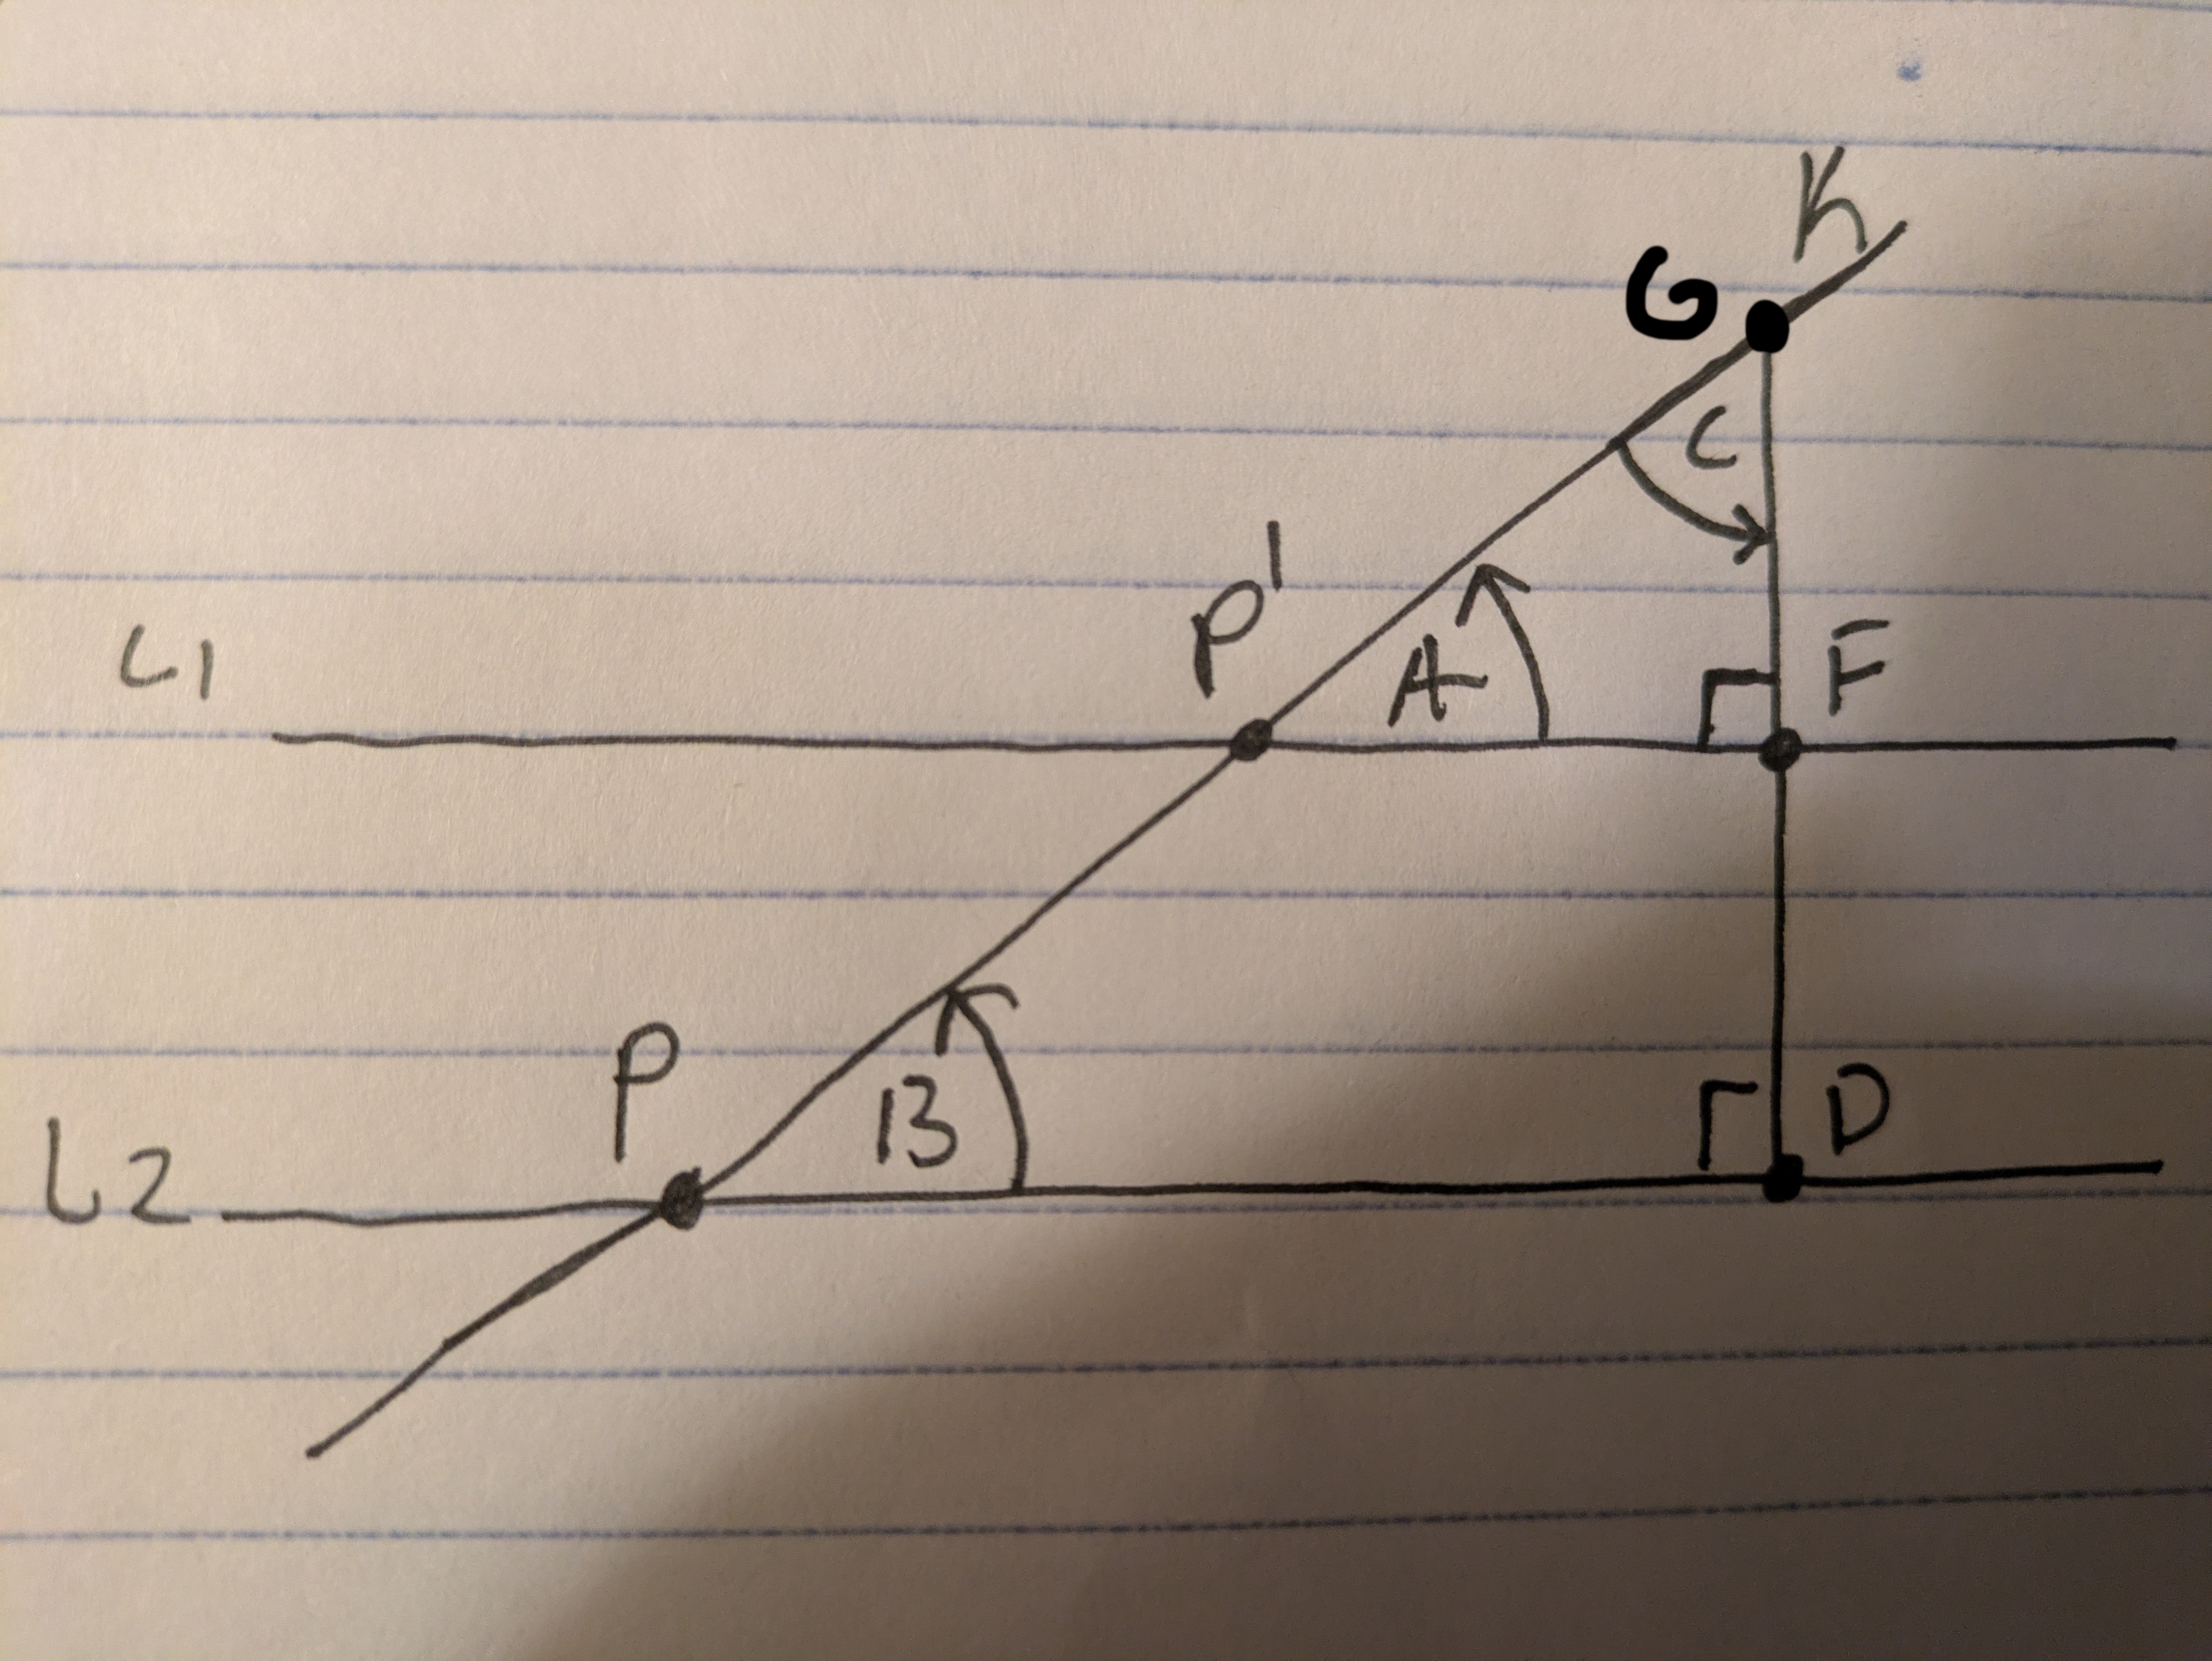
\includegraphics[width=0.6\textwidth]{images/5_5_a.jpg}
\end{figure}

\begin{figure}[h]
    \centering
    \includegraphics[width=0.6\textwidth]{images/5_again.png}
\end{figure}

\begin{figure}[h]
    \centering
    \includegraphics[width=0.6\textwidth]{images/lets_go.png}
\end{figure}

\begin{proof}
    Refer to the figure. Consider the areas enclosed by the right triangles 
        $\triangle P'FG$ and $\triangle PDG$.
    By Problem $10$, the degrees of $\triangle P'FG$ is $90\textdegree + m(A) + m(C) = 180\textdegree$.
    Similarly, the degress of $\triangle PDG$ is $90\textdegree + m(B) + m(C) = 180\textdegree$.
    Then $90\textdegree + m(A) + m(C) = 90\textdegree + m(B) + m(C)$
        and it follows that $m(A) = m(B)$.
\end{proof}

\begin{proof}
    Refer to the text. Then let the parallel segments formed by points $Q, P$ and $N, M$
        be the parallel lines $L_1$, $L_2$. Also let $B$ be the $B$ in our problem.
    Finally, let $\angle NQM$ be $m(B')$.
    It then follows from the text that $m(B) = m(B')$.
\end{proof}

\begin{proof}
    Refer to the figure. Line $D$ is parallel to line $K$.
    The measure of the green angle is equal to $m(A)$ by Problem $13$(b).
    Then $m(A') = m(A)$ by Problem $13$(a).
\end{proof}

\section{Mathematical Induction}
\begin{tcolorbox}[title=Problem 1, breakable]
    Show that in a ring, $0a = a0 = 0$.
\end{tcolorbox}

\begin{proof}
    Let $R$ be a ring and $a$ be an arbitrary element in $R$.
    Then
    \begin{align*}
        0a &= 0a + 0 &&\text{Rule 3} \\
            &= 0a + (0a + (-0a)) &&\text{Rule 4} \\
            &= (0a + 0a) + (-0a) &&\text{Rule 2} \\
            &= ((0 + 0)a) + (-0a) &&\text{Rule 6} \\
            &= 0a + (-0a) &&\text{Rule 3} \\
            &= 0 &&\text{Rule 3}
    \end{align*}
    Similarly 
    \begin{align*}
        a0 &= a0 + 0 &&\text{Rule 3} \\
            &= a0 + (a0 + (-a0)) &&\text{Rule 4} \\
            &= (a0 + a0) + (-a0) &&\text{Rule 2} \\
            &= (a(0 + 0)) + (-a0) &&\text{Rule 6} \\
            &= a0 + (-a0) &&\text{Rule 3} \\
            &= 0 &&\text{Rule 3}
    \end{align*}
    Thus $a0 = 0a = 0$.
\end{proof}

\begin{tcolorbox}[title=Problem 2, breakable]
    Prove part d of Theorem 6.1:
    Show that in a ring the additive identity is unique,
        by supposing $0$ and $0'$ satisfy Rule 3
        and proving that $0 = 0'$.
\end{tcolorbox}

\begin{proof}
    Let $R$ be a ring and suppose there exists $0 \in R$
        and $0' \in R$ such that 
        for all $a \in R$, $a + 0 = a$ and $a + 0' = a$.
    Then $a + 0 = a = a + 0'$.
    By Additive Cancellation $0 = 0'$.
\end{proof}

\begin{tcolorbox}[title=Problem 3, breakable]
    Show that in a ring $(-a)b = a(-b) = -(ab)$.
\end{tcolorbox}

\begin{proof}
    Let $R$ be a ring and $a, b \in R$. Then
    \begin{align*}
        0 = (a + (-a))b 
        \iff &0 = ab + (-a)b &&\text{Rule 6} \\
        \iff &-(ab) + 0 = -(ab) + (ab + (-a)b) \\
        \iff &-(ab) = -(ab) + (ab + (-a)b) &&\text{Rule 3} \\
        \iff &-(ab) = (-(ab) + ab) + (-a)b &&\text{Rule 2} \\
        \iff &-(ab) = 0 + (-a)b &&\text{Rule 4} \\
        \iff &-(ab) = (-a)b + 0 &&\text{Rule 1} \\
        \iff &-(ab) = (-a)b &&\text{Rule 3}
    \end{align*}
    Also
    \begin{align*}
        0 = a(b + (-b)) 
        \iff &0 = ab + a(-b) &&\text{Rule 6} \\
        \iff &-(ab) + 0 = -(ab) + ((ab) + a(-b))  \\
        \iff &-(ab) = -(ab) + ((ab) + a(-b)) &&\text{Rule 3} \\
        \iff &-(ab) = (-(ab) + (ab)) + a(-b) &&\text{Rule 2} \\
        \iff &-(ab) = 0 + a(-b) &&\text{Rule 4} \\
        \iff &-(ab) = a(-b) + 0 &&\text{Rule 1} \\
        \iff &-(ab) = a(-b) &&\text{Rule 3}
    \end{align*}
    Thus $(-a)b = a(-b) = -(ab)$.
\end{proof}

\begin{tcolorbox}[title=Problem 4, breakable]
    Show that in a ring $(-a)(-b) = ab$.
\end{tcolorbox}

\begin{proof}
    \begin{align*}
        (-a)(-b) + -(ab) &= a(-(-b)) + a(-b) && \text{Rule 6} \\
                        &= a((-(-b)) + (-b)) && \text{Rule 2} \\
                        &= a \cdot 0 && \text{Rule 4} \\
                        &= 0 && \text{Rule 3}
    \end{align*}
    Thus $(-a)(-b) = ab$.
\end{proof}

\begin{tcolorbox}[title=Problem 5, breakable]
    Prove the following facts about subtraction in a ring $R$,
    where $a, b, c \in R$.

    (a) $a - a = 0$.

    (b) $a(b - c) = ab - ac$.

    (c) $(b - c)a = ba - ca$.
\end{tcolorbox}

\begin{proof}
    Let $R$ be a ring and $a, b, c \in R$.
    Then $a - a = a + (-a) = 0$ Rule 4.
    Also, $a(b - c) = a(b + (-c)) = ab + a(-c)$ Rule 6.
    Then, $ab + a(-c) = ab + -(ac) \text{ Problem 3 } = ab - ac$.
    Similarly, $(b - c)a = (b + (-c))a = ba + (-c)a$ Rule 6.
    Then, $ba + (-c)a = ba + -(ca) \text{ Problem 3 } = ba - ca$.
\end{proof}

\begin{tcolorbox}[title=Problem 8, breakable]
    We generalize Exercises 6 and 7: Let $R$
    be any commutative ring (other than the zero ring).
    Define $M_2(R)$ as the set of $2 \times 2$
    matrices with entries from $R$. Show that $M_2(R)$
    is a ring which is not commutative. (Note that 
    for the most part the proofs in Exercises 6 and 
    7 life over without change.)
\end{tcolorbox}

\begin{proof}
    Let $R$ be a ring and 
    \[a, b, c, e, f, g, h, i, j, k, l \in R\]
    We first show associativity with respect to $+$.
    \[\begin{bmatrix}
        a & b \\
        c & d
    \end{bmatrix} \in M_2(R) \text{, }
    \begin{bmatrix}
        c & f \\
        g & h
    \end{bmatrix} \in M_2(R) \text{ and }
    \begin{bmatrix}
        i & j \\
        k & l
    \end{bmatrix} \in M_2(R)\]
    Then 
    \[\begin{bmatrix}
        a & b \\
        c & d
    \end{bmatrix} + \begin{bmatrix}
        c & f \\
        g & h
    \end{bmatrix} = \begin{bmatrix}
        a+c & b+f \\
        c+g & d+h
    \end{bmatrix} = \begin{bmatrix}
        c+a & f+b \\
        g+c & h+d
    \end{bmatrix} = \begin{bmatrix}
        c & f \\
        g & h
    \end{bmatrix} + \begin{bmatrix}
        a & b \\
        c & d
    \end{bmatrix}\]
    We now show associativity with respect to $+$.
\[\left(\begin{bmatrix}
        a & b \\
        c & d
    \end{bmatrix} + \begin{bmatrix}
        c & f \\
        g & h
    \end{bmatrix}\right) + \begin{bmatrix}
        i & j \\
        k & l
    \end{bmatrix} = \begin{bmatrix}
        a+c & b+f \\
        c+g & d+h
    \end{bmatrix} +\begin{bmatrix}
        i & j \\
        k & l
    \end{bmatrix} = \begin{bmatrix}
        (a+c)+i & (b+f)+j \\
        (c+g)+k & (d+h)+l
    \end{bmatrix}\] \[= \begin{bmatrix}
        a+(c+i) & b+(f+j) \\
        c+(g+k) & d+(h+l)
    \end{bmatrix} = \begin{bmatrix}
        a & b \\
        c & d
    \end{bmatrix} + \begin{bmatrix}
        c+i & f+j \\
        g+k & h+l
    \end{bmatrix} = \begin{bmatrix}
        a & b \\
        c & d
    \end{bmatrix} + \left(\begin{bmatrix}
        c & f \\
        g & h
    \end{bmatrix} + \begin{bmatrix}
        i & j \\
        k & l
    \end{bmatrix}\right)\]
    We now show the existence of an additive inverse.
    \[\begin{bmatrix}
        a & b \\
        c & d
    \end{bmatrix} -\begin{bmatrix}
        a & b \\
        c & d
    \end{bmatrix} = \begin{bmatrix}
        a-a & b-b \\
        c-c & d-d
    \end{bmatrix} = \begin{bmatrix}
        0 & 0 \\
        0 & 0
    \end{bmatrix}\]
    We now show the existence of the additive identity.
    \[\begin{bmatrix}
        a & b \\
        c & d
    \end{bmatrix} + \begin{bmatrix}
        0 & 0 \\
        0 & 0
    \end{bmatrix} = \begin{bmatrix}
        a+0 & b+0 \\
        c+0 & d+0
    \end{bmatrix} = \begin{bmatrix}
        a & b \\
        c & d
    \end{bmatrix}\]
    We now show left distributivity.
    \[
    \begin{bmatrix}
        a & b \\
        c & d
    \end{bmatrix}
    \left(
    \begin{bmatrix}
        e & f \\
        g & h
    \end{bmatrix}
    +
    \begin{bmatrix}
        i & j \\
        k & l
    \end{bmatrix}
    \right)
    =
    \begin{bmatrix}
        a & b \\
        c & d
    \end{bmatrix}
    \begin{bmatrix}
        e+i & f+j \\
        g+k & h+l
    \end{bmatrix}
    =
    \begin{bmatrix}
        a(e+i) + b(g+k) & a(f+j) + b(h+l) \\
        c(e+i) + d(g+k) & c(f+j) + d(h+l)
    \end{bmatrix}
    \]
    \[
    =
    \begin{bmatrix}
        ae + bg & af + bh \\
        ce + dg & cf + dh
    \end{bmatrix}
    +
    \begin{bmatrix}
        ai + bk & aj + bl \\
        ci + dk & cj + dl
    \end{bmatrix}
    =
    \begin{bmatrix}
        a & b \\
        c & d
    \end{bmatrix}
    \begin{bmatrix}
        e & f \\
        g & h
    \end{bmatrix}
    +
    \begin{bmatrix}
        a & b \\
        c & d
    \end{bmatrix}
    \begin{bmatrix}
        i & j \\
        k & l
    \end{bmatrix}.
    \]
    We now show right distributivity.
    \[
    \left(
    \begin{bmatrix}
        e & f \\
        g & h
    \end{bmatrix}
    +
    \begin{bmatrix}
        i & j \\
        k & l
    \end{bmatrix}
    \right)
    \begin{bmatrix}
        a & b \\
        c & d
    \end{bmatrix}
    =
    \begin{bmatrix}
        e+i & f+j \\
        g+k & h+l
    \end{bmatrix}
    \begin{bmatrix}
        a & b \\
        c & d
    \end{bmatrix}
    =
    \begin{bmatrix}
        (e+i)a + (f+j)c & (e+i)b + (f+j)d \\
        (g+k)a + (h+l)c & (g+k)b + (h+l)d
    \end{bmatrix}
    \]
    \[
    =
    \begin{bmatrix}
        ea + fc & eb + fd \\
        ga + hc & gb + hd
    \end{bmatrix}
    +
    \begin{bmatrix}
        ia + jc & ib + jd \\
        ka + lc & kb + ld
    \end{bmatrix}
    =
    \begin{bmatrix}
        e & f \\
        g & h
    \end{bmatrix}
    \begin{bmatrix}
        a & b \\
        c & d
    \end{bmatrix}
    +
    \begin{bmatrix}
        i & j \\
        k & l
    \end{bmatrix}
    \begin{bmatrix}
        a & b \\
        c & d
    \end{bmatrix}
    \]
    We now show matrix multiplication is not commutative 
        by giving a counterexample.
    Consider
    \[
    \begin{bmatrix}
    1 & 2 \\
    0 & 1
    \end{bmatrix}
    \begin{bmatrix}
    1 & 0 \\
    3 & 1
    \end{bmatrix}
    =
    \begin{bmatrix}
    1+6 & 2 \\
    3 & 1
    \end{bmatrix}
    =
    \begin{bmatrix}
    7 & 2 \\
    3 & 1
    \end{bmatrix}
    \]
    But multiplying the same matrices in the opposite order gives
    \[
    \begin{bmatrix}
    1 & 0 \\
    3 & 1
    \end{bmatrix}
    \begin{bmatrix}
    1 & 2 \\
    0 & 1
    \end{bmatrix}
    =
    \begin{bmatrix}
    1 & 2 \\
    3 & 7
    \end{bmatrix}.
    \]
    Since
    \[
    \begin{bmatrix}
    7 & 2 \\
    3 & 1
    \end{bmatrix}
    \neq
    \begin{bmatrix}
    1 & 2 \\
    3 & 7
    \end{bmatrix}
    \]
    matrix multiplication is not commutative.
\end{proof}

Let $R = \{0, a, \ldots\}$ such that $0 \ne a$.
\[
A = \begin{bmatrix} 0 & a \\ 0 & 0 \end{bmatrix}, \quad
B = \begin{bmatrix} 0 & 0 \\ a & 0 \end{bmatrix}
\]
\[
AB = \begin{bmatrix} a^2 & 0 \\ 0 & 0 \end{bmatrix} \neq 
BA = \begin{bmatrix} 0 & 0 \\ 0 & a^2 \end{bmatrix}
\]

\begin{tcolorbox}[title=Problem 9, breakable]
    Check that Example 6.14 is indeed a ring; that is,
    let $C[0, 1]$ be a set of functions defined from the closed 
    unit interval $[0, 1]$ to the real numbers that 
    are continuous. Define the sum and product of two 
    functions point-wise: $(f + g)(x) = f(x) + g(x)$
    and $(fg)(x) = f(x)g(x)$. Show that $C[0, 1]$ is a 
    commutative ring. (You may use theorems from calculus).
\end{tcolorbox}

\begin{proof}
    Let $x \in [0, 1]$ and $f, g, l : [0, 1] \longrightarrow \mathbb{R}$.
    Since $f(x), g(x), l(x) \in \mathbb{R}$ and $\mathbb{R}$ is a ring, standard ring operations (associativity, distributivity, etc.) hold.
    We first show commutativity over addition
    \[
    (f + g)(x) = f(x) + g(x) = g(x) + f(x) = (g + f)(x)
    \]
    Next, associativity over addition
    \[
    ((f + g) + l)(x) = (f + g)(x) + l(x) = f(x) + g(x) + l(x) = f(x) + (g + l)(x) = (f + (g + l))(x).
    \]
    Existence of additive inverses
    \[
    (f + (-f))(x) = f(x) + (-f(x)) = 0
    \]
    Additive identity
    \[
    (f + 0)(x) = f(x) + 0(x) = f(x)
    \]
    Commutativity of multiplication
    \[
    (fg)(x) = f(x) g(x) = g(x) f(x) = (gf)(x)
    \]
    Associativity of multiplication
    \[
    ((fg)l)(x) = (fg)(x) l(x) = f(x) g(x) l(x) = f(x) (gl)(x) = (f(gl))(x)
    \]
    Distributivity from the left
    \[
    f(g + l)(x) = f(x)(g + l)(x) = f(x)(g(x) + l(x)) = f(x)g(x) + f(x)l(x) = (fg + fl)(x)
    \]
    Distributivity from the right
    \[
    (f + g)l(x) = (f + g)(x) \, l(x) = (f(x) + g(x))l(x) = f(x)l(x) + g(x)l(x) = (fl + gl)(x)
    \]
\end{proof}

\begin{tcolorbox}[title=Problem 11, breakable]
    Let $\mathbb{C}$ be the complex numbers. That inverse
    \[\mathbb{C} = \{a + bi \mid a, b, \in \mathbb{R}\}\]
    where $i$ is the square root of $-1$ (that is, $i \cdot i = 1$).
    Here 
    \[(a + bi) + (c + di) = (a + c) + (bi + di)\]
    and 
    \[(a + bi)(c + di) = (ac - bd) + (ad + bc)i\]
    Show that $\mathbb{C}$ is a commutative ring.
\end{tcolorbox}

\begin{proof}
    Let $a + bi, c + di, e + fi \in \mathbb{C}$.
    We first show commutativity over addition
    \[
    (a + bi) + (c + di) = (a + c) + (bi + di) = (c + a) + (di + bi) = (c + di) + (a + bi)
    \]
    Next, associativity over addition
    \[
    ((f + g) + l)(x) = (f + g)(x) + l(x) = f(x) + g(x) + l(x) = f(x) + (g + l)(x) = (f + (g + l))(x).
    \]
    Existence of additive inverses
    \[
    (f + (-f))(x) = f(x) + (-f(x)) = 0
    \]
    Additive identity
    \[
    (f + 0)(x) = f(x) + 0(x) = f(x)
    \]
    Commutativity of multiplication
    \[
    (fg)(x) = f(x) g(x) = g(x) f(x) = (gf)(x)
    \]
    Associativity of multiplication
    \[
    ((fg)l)(x) = (fg)(x) l(x) = f(x) g(x) l(x) = f(x) (gl)(x) = (f(gl))(x)
    \]
    Distributivity from the left
    \[
    f(g + l)(x) = f(x)(g + l)(x) = f(x)(g(x) + l(x)) = f(x)g(x) + f(x)l(x) = (fg + fl)(x)
    \]
    Distributivity from the right
    \[
    (f + g)l(x) = (f + g)(x) \, l(x) = (f(x) + g(x))l(x) = f(x)l(x) + g(x)l(x) = (fl + gl)(x)
    \]
\end{proof}

\begin{tcolorbox}[title=Problem 15, breakable]
    Verify that 6.10 is a ring.
    Namely, let $R$ and $S$ be arbitrary rings.
    Define addition and subtraction appropriately
        to make $R \times S$ a ring,
        where $R \times S$ is the set of ordered pairs
        with the first entry from $R$ and second entry 
        from $S$. 
    Now generalize this to the set $R_1 \times R_2 \times \cdots R_n$
    of $n$-tuples with entries from the rings $R_i$.
    This new ring is called the \textbf{direct product}
    of the rings $R_i$.
\end{tcolorbox}

\end{document}
